\documentclass[tikz,12pt,margin=0px]{article}

\usepackage[a4paper,bindingoffset=0.2in,
            left=1.5cm,right=1.5cm,top=1.25cm,bottom=1.5cm,%
            footskip=.35in]{geometry}
\usepackage[normalem]{ulem}
\usepackage[utf8]{inputenc}
\usepackage{amsmath}
\usepackage{amssymb}
\usepackage{collectbox}
\usepackage{comment}
\usepackage{enumitem}
\usepackage{fancyhdr}
\usepackage{float}
\usepackage{fontawesome}
\usepackage{makecell}
\usepackage{pgfplotstable}
\usepackage{tikz}
\usepackage{titlesec}
\usepackage[magyar]{babel}

\usetikzlibrary{positioning,calc,shapes.multipart,arrows,arrows.meta,matrix,automata,shapes.misc}

\setlist[itemize,1]{label=$\bullet$}
\setlist[itemize,2]{label=$\circ$}
\setlist[itemize,3]{label=$\centerdot$}
\setlist[itemize,4]{label=$\cdot$}

\titleformat*{\section}{\Large\bfseries}
\titleformat*{\subsection}{\large\bfseries}
\titleformat*{\subsubsection}{\normalsize\bfseries}
\titleformat*{\paragraph}{\small\bfseries}
\titleformat*{\subparagraph}{\footnotesize\bfseries}

\newcommand\ddfrac[2]{\frac{\displaystyle #1}{\displaystyle #2}}

\newcommand{\mybox}{%
    \collectbox{%
        \setlength{\fboxsep}{4pt}%
        \fbox{\BOXCONTENT}%
    }%
}

 \geometry{
 a4paper,
 total={170mm,257mm},
 left=20mm,
 right=20mm,
 top=20mm,
 bottom=20mm
 }

\setlist[itemize,1]{label=$\bullet$}
\setlist[itemize,2]{label=$\circ$}
\setlist[itemize,3]{label=$\centerdot$}
\setlist[itemize,4]{label=$\cdot$}

\pagestyle{fancy}

\newcommand\blfootnote[1]{%
  \begingroup
  \renewcommand\thefootnote{}\footnote{#1}%
  \addtocounter{footnote}{-1}%
  \endgroup
}

\renewcommand{\figurename}{ábra}
\newenvironment{tetel}[1]{\paragraph{#1 \\}}{}

\newcommand{\N}{\mathbb{N}}
\newcommand{\Z}{\mathbb{Z}}
\newcommand{\R}{\mathbb{R}}
\newcommand{\Q}{\mathbb{Q}}
\newcommand{\C}{\mathbb{C}}

\makeatletter
\renewcommand\paragraph{%
	\@startsection{paragraph}{4}{0mm}%
	{-\baselineskip}%
	{.5\baselineskip}%
	{\normalfont\normalsize\bfseries}}
\makeatother
\newcommand\lword[1]{\leavevmode\nobreak\hskip0pt plus\linewidth\penalty50\hskip0pt plus-\linewidth\nobreak #1}

\useunder{\uline}{\ul}{}
\fancyhead{}
\cfoot{3. tétel | \thepage. oldal}

\renewcommand{\headrulewidth}{0pt}
\renewcommand{\footrulewidth}{0.4pt}

\begin{document}
    \thispagestyle{fancy}
    \hyphenation{oddword}
    \uchyph=0
    \begin{center}
        {\Large\bfseries\noindent 3. Numerikus módszerek} \\
    \end{center}
	
	\section*{Iterációs módszerek: Lineáris egyenletrendszerekre és nemlineáris egyenletekre.}
	
    \textbf{Definíció.} Egy $m$ egyenletből álló, $n$-ismeretlenes \emph{lineáris egyenletrendszer általános alakja}:
    \[
          \begin{array}{ccccccccc}
            a_{11}x_{1} & + & a_{12}x_{2} & + & \ldots & + & a_{1n}x_{n} & = & b_{1} \\
            a_{21}x_{1} & + & a_{22}x_{2} & + & \ldots & + & a_{2n}x_{n} & = & b_{2} \\
              &   &   &   &   &   & \vdots  & \vdots & \vdots \\
            a_{m1}x_{1} & + & a_{m2}x_{2} & + & \ldots & + & a_{mn} & = & b_{m} \\
          \end{array}
    \]

    \noindent Az egyenletrendszer átírható $A\underline{x} = \underline{b}$ formába is, ahol\\
    \[
        A = \left(
              \begin{array}{cccc}
                a_{11} & a_{12} & \ldots & a_{1n} \\
                a_{11} & a_{22} & \ldots & a_{2n} \\
                \vdots & \vdots & \ddots & \vdots \\
                a_{m1} & a_{m2} & \ldots & a_{mn} \\
              \end{array}
            \right), \quad
        \underline{x} = \left(
              \begin{array}{c}
                x_{1} \\
                x_{2} \\
                \vdots \\
                x_{m} \\
              \end{array}
            \right), \quad
        \underline{b} = \left(
              \begin{array}{c}
                b_{1} \\
                b_{2} \\
                \vdots \\
                b_{m} \\
              \end{array}
            \right)
    \]\\

    \noindent Az $a_{ij}$ együtthatókból képzett $A$ mátrixot az egyenletrendszer \emph{együtthatómátrixa}. Ha ezt kibővítjük a $\underline{b}$ vektor $b_{i}$ komponenseiből képzett oszlopvektorral, akkor az egyenletrendszer $m \times (n+1)$-es \emph{kibővített mátrixát} kapjuk, amit $A|\underline{b}$-vel jelölünk.\\
    \[
        A|\underline{b} = \left(
              \begin{array}{ccccc}
                a_{11} & a_{12} & \ldots & a_{1n} & b_{1} \\
                a_{11} & a_{22} & \ldots & a_{2n} & b_{2} \\
                \vdots & \vdots & \ddots & \vdots & \vdots \\
                a_{m1} & a_{m2} & \ldots & a_{mn} & b_{n} \\
              \end{array}
            \right)
    \]\\

    \noindent \textbf{Tétel 1.} (Kronecker–Capelli-tétel): Az $A\underline{x} = \underline{b}$ \emph{akkor és csak akkor megoldható}, ha az $A$ együtthatómátrix és az $A|\underline{b}$ kibővített mátrix rangja megegyezik: $\boldsymbol{r(A) = r(A|\underline{b})}$.\\

    \noindent \textbf{Tétel 2.} Ha az egyenletrendszer megoldható és
    \begin{itemize}
        \item $r(A) < n$, akkor végtelen sok megoldás van, ha
        \item $r(A)=n$, akkor egyértelmű a megoldás.
    \end{itemize}

	\section*{Lineáris egyenletrendszerek iterációs módszerei}

    \noindent A lineáris algebrai egyenletrendszerek megoldási módszerei:\emph{direkt} illetve az \emph{iterációs módszerek}. Direkt módszereknek azokat a módszereket nevezzük, amelyekkel pontosan számolva az egyenletrendszer pontos megoldását kapnánk. Ezek közé tartoznak az eliminációs módszerek, a felbontási módszerek és a Cramer-szabály. Hátrányuk, hogy csak kisebb méretű egyenletrendszerek oldhatók meg velük reális időn belül. Így a gyakorlati feladatok esetén (amelyekben gyakran nagy méretű az együtthatómátrix) az iterációs módszereket használjuk, melyek nagy előnye a direkt módszerekkel szemben a kisebb tárigény, valamint kihasználhatók a gyakran meglévő hozzávetőleges információk is a megoldás várható értékeiről.\\

    \noindent Tegyük fel, hogy az $A\underline{x}=\underline{b}$ egyenletrendszer együtthatómátrixa négyzetes ($A \in \mathbb{R}^{n \times n}$) és determinánsa nullától különbözik ($det A \neq 0$). Ekkor az 2. tételből következően az egyenletrendszernek egyetlen megoldása létezik. Az iterációs módszerek ezen egyértelmű megoldás közelítő meghatározására adnak lehetőséget.\\

    \noindent Az iterációs módszerek általában olyan konvergens sorozatot konstruálnak, melyek határértéke az egyenletrendszer megoldása.\\

	\noindent A lineáris egyenletrendszert (LER) vektorsorozatokkal közelítjük, törekedve a minél gyorsabb konvergenciára.
	Az iterációs módszereknek a lényege a következő átalakítás:
    \[
        \mybox{$A\underline{x} = \underline{b} \Longleftrightarrow \underline{x} = B\underline{x} + \underline{r}$}
    \]
    Ilyen alak létezik,	sőt nem egyértelmű,	hanem sokféle lehet, és a különböző átalakítások szolgáltatják a különféle iterációs módszereket. A $B$-t \emph{átmenetmátrixnak} nevezzük.\\

	\noindent \textbf{Kontrakció}: A $\varphi: \mathbb{R}^{n} \to \mathbb{R}^{n}$ függvény \emph{kontrakció}, ha
    \begin{center}
        $\exists 0 \leq q < 1 : \forall \underline{x}, \underline{y} \in \mathbb{R}^{n}: \Vert \varphi(\underline{x}) - \varphi(\underline{y}) \Vert \leq q \Vert \underline{x} - \underline{y} \Vert$
	\end{center}
	\noindent A $q$ értéket \emph{kontrakciós együtthatónak} nevezzük.\\

    \noindent Példa kontrakcióra: $\ddfrac{1}{2}\cos x,\ x \in [0,\ddfrac{\pi}{2}]$ \Big| $\ddfrac{3 - x^2}{3},\ x \in [0,1]$ \Big| $2 + e^{-x},\ x \in [1, +\infty)$.\\

	\noindent \textbf{Banach-féle fixponttétel}: Legyen $\varphi: \mathbb{R}^{n} \to \mathbb{R}^{n}$ kontrakció a $q$
	kontrakciós együtthatóval.\\

    \noindent Ekkor a következő állítások igazak:
	
	\begin{enumerate}
		\item $\exists! \underline{x}^{*} \in \mathbb{R}^{n}: \underline{x}^{*} = \varphi(\underline{x}^{*})$. Azt mondjuk, hogy $\underline{x}^{*}$ az $\varphi$ függvény
		fixpontja.
		
        \item $\forall \underline{x}^{(0)} \in \mathbb{R}^{n}$ kezdőérték esetén az $\underline{x}^{(k+1)} = \varphi(\underline{x}^{(k)}) \quad (k \in \mathbb{N})$ rekurzióval definiált sorozat konvergens, és a határértéke az $\underline{x}^{*}$, azaz
        \[
            \lim \limits_{k\to\infty} \underline{x}^{(k)} = \underline{x}^{*}
        \]
		
		\item teljesül az alábbi hibabecslés:
        \begin{center}
    	   $\Vert \underline{x}^{(k)} - \underline{x}^{*}\Vert \leq \ddfrac{q^{k}}{1-q} \Vert \underline{x}^{(1)} - \underline{x}^{(0)}\Vert$.
        \end{center}
	\end{enumerate}
	
    \noindent Az egyenletrendszer megoldása így az $\varphi: \mathbb{R}^{n} \rightarrow \mathbb{R}^{n},\ \varphi(\underline{x}) = B\underline{x} + \underline{r}$ függvény fixpontjának keresésére vezethető vissza.\\

    \noindent Ez esetben tehát csak azt kell biztosítani, hogy $\varphi$ kontrakció legyen, és csak alkalmazni kell rá a fixpont tételt.
    \[
        \boldsymbol{\Vert \varphi(x) - \varphi(y) \Vert} = \Vert B\underline{x} + \underline{r} - (B\underline{y}+\underline{r}) \Vert = \Vert B\underline{x} - B\underline{y} \Vert \boldsymbol{= \Vert B(\underline{x} - \underline{y}) \Vert \leq \Vert B \Vert \Vert x - y \Vert}
    \]

    \noindent Tehát, ha a $B$ mátrix valamely indukált vagy illeszkedő normája kisebb egynél, akkor az $\varphi$ függvény kontrakció, és a fixponttétel alkalmazható.\\
\newpage
    \noindent \textbf{Tétel:} (\textbf{\emph{Elégséges feltétel a konvergenciára}}): Ha a lineáris egyenletrendszer $B$ \lword{átmenetmátrixára} $\Vert B \Vert < 1$, akkor tetszőleges $\underline{x}^{(0)}$-ból indított $\underline{x}^{(k+1)} := B\underline{x}^{(k)} + \underline{r}$ iteráció konvergál az $A\underline{x} = \underline{b}$ lineáris egyenletrendszer megoldásához.\\

    \noindent A konvergencia vizsgálatakor lehet, hogy a fenti elégséges feltétel nem teljesül, ezért nézzük a konvergencia szükséges és elégséges feltételét.\\

    {\footnotesize \noindent {\color{blue} \faLightbulbO\ $\triangleright$ } }
    {\footnotesize
    \noindent \textbf{Lemma.} Legyen $B \in \mathbb{R}^{n \times n}$. Ekkor $\forall \varepsilon > 0$ esetén $\exists \Vert B \Vert$ indukált norma, úgy hogy
    \[
        \Vert B \Vert < \rho(B) + \varepsilon
    \]

    \noindent ahol $\rho(B)$ a $B$ mátrix spektrálsugara, vagyis

    \[
        \rho(B) = \inf\limits_{\Vert \ \Vert \text{indukált}} \Vert B \Vert \qquad \forall B \in \mathbb{R}^{n \times n}
    \]
    \noindent $\triangleleft$ \faLightbulbO}\\

	\noindent \textbf{Tétel:} (\textbf{\emph{Szükséges és elégséges feltétel a konvergenciára}}):
    Tetszőleges $\underline{x}^{(0)} \in \mathbb{R}^{n}$-ból indított $\underline{x}^{(k+1)} := B\underline{x}^{(k)} + \underline{r}$ iteráció konvergál az $A\underline{x} = \underline{b}$ lineáris egyenletrendszer megoldásához $\Longleftrightarrow \rho(B) < 1$.\\

    \noindent Tehát a következőkben a különböző iterációs eljárások esetén az $\underline{x} = B\underline{x} + \underline{r}$ átalakítás után képezzük az $\underline{x}^{(k+1)} = B\underline{x}^{(k)} + \underline{r}$ iterációt valamilyen $\underline{x}^{(0)}$ kezdőértékkel.

	\subsection*{Jacobi-iteráció}
	
    \noindent Vegyük az $A\underline{x}=\underline{b}$ egyenletrendszert, és tegyük fel, hogy $A \in \mathbb{R}^{n \times n}$ és $det(A) \neq 0$. Ekkor az egyenletrendszernek létezik egyértelmű megoldása.\\

    \noindent Írjuk fel az egyenletrendszer komponensenkénti alakját:
    \begin{center}
        $A\underline{x}=\underline{b} \Leftrightarrow a_{i,1}x_1 + \ldots + a_{i,n}x_{n} = b_i\qquad (i = 1, \ldots, n) \quad (1)$
    \end{center}

    \noindent Tegyük fel, hogy $a_{ii} \neq 0 \quad (i = 1, \ldots, n)$.\\

    \noindent Ekkor az $(1)$ átírható $a_{ii}$-vel leosztva és átrendezve:
    \[
        x_{i} = -\Big[\ddfrac{a_{i,1}}{a_{i,i}}x_1 + \ddfrac{a_{i,2}}{a_{i,i}}x_2 + \cdots + \ddfrac{a_{i,i-1}}{a_{i,i}}x_{i-1}  + \ddfrac{a_{i,i+1}}{a_{i,i}}x_{i+1} + \cdots + \ddfrac{a_{i,n}}{a_{i,i}}x_{n} \Big] + \ddfrac{b_{i}}{a_{i,i}} \qquad (\forall i = 1, \ldots, n)
    \]

    \noindent Ebből felépíthető egy iteráció, ahol $x_{i}^{(k)}$ az $i$-edik ismeretlen $k$-adik közelítése:
    \[
        x_{i}^{(k+1)} = -\Big[\ddfrac{a_{i,1}}{a_{i,i}}x_1^{(k)} + \cdots + \ddfrac{a_{i,n}}{a_{i,i}}x_n^{(k)}\Big] + \ddfrac{b_{i}}{a_{i,i}}\quad {\small\text{ahol}\ x_{i}^{(0)}\ \text{tetszőleges érték és}\ k = 0, 1, \ldots.}
    \]

    \noindent Összevont alakban:
	\begin{displaymath}
    \mybox{
		$\boldsymbol{\underline{x}^{(k+1)}_{i}} :=
		-\ddfrac{1}{a_{i,i}}
		\Bigg(
		\sum_{\substack{j=1\\ j \not = i}}^{n} a_{i,j}\boldsymbol{\underline{x}_{j}^{(k)}} - \underline{b}_{i}
		\Bigg)
		\; (i = 1, \ldots, n)$
    }
	\end{displaymath}

    \noindent Az iteráció felírható mátrixos alakban is. Továbbra is $det(A) \neq 0$. Ekkor létezik legalább egy elemi szorzata a mátrixnak - a determináns definíciója - szerint, amelyik nem nulla, így pusztán sorcserével elérhető, hogy az $A$ mátrix diagonálisában csupa nemnulla elem álljon.\\

    \noindent Ekkor az $A$ mátrixnak elkészíthető a következő felbontása
    \[
        A = L + D + U
    \]
    ahol \emph{L}: alsó háromszög mátrix, \emph{D}: diagonális mátrix, \emph{U}: felső háromszög mátrix.\\

	\noindent Ekkor azonos átalakításokkal a következő relációk érvényesek:
	
	\begin{center}
		$A\underline{x} = \underline{b} \Leftrightarrow (L + D + U)\underline{x} = \underline{b}$ \\
        $D\underline{x} = -(L+U)\underline{x}+\underline{b}$ \\
		$\underline{x} = -D^{-1}(L+U)\underline{x} + D^{-1}\underline{b}$
	\end{center}
	
    \noindent Ebből már származtatható a Jacobi-iteráció mátrixos alakja:
    \begin{center}
        \mybox{
        $\underline{x}^{(k+1)} = \underbrace{-D^{-1}(L + U)}_{:= B_{J}}\underline{x}^{(k)} + \underbrace{D^{-1}\underline{b}}_{:= r_{J}}$
        }
    \end{center}
	\noindent $B_{J}$ a Jacobi-iteráció \emph{iterációs mátrixát} jelöli.\\

    \subsubsection*{A Jacobi-iteráció konvergenciája\\}

    {\footnotesize \noindent {\color{blue} \faLightbulbO\ $\triangleright$ } }
    {\footnotesize
    \noindent \textbf{Definíció.} Az A mátrix \emph{szigorúan diagonálisan domináns}, ha minden sorban a főátlóban lévő eleme nagyobb, mint az adott sorban lévő összes többi elem abszolút értékének összege, azaz
    \[
        |a_{i,i}| > \sum_{\substack{j=1\\ j \not = i}}^{n} |a_{i,j}|\quad (i = 1, 2, \ldots, n)
    \]
    \noindent $\triangleleft$ \faLightbulbO}\\

    \noindent \textbf{Tétel}: Ha az $Ax = b$ lineáris egyenletrendszer mátrixa szigorúan diagonálisan domináns akkor a Jakobi-iteráció konvergens.\\

    \noindent A Jakobi iteráció konvergál, ha $||B_{J}|| < 1$, valamely indukált vagy illeszkedő normában (elégséges feltétel).

\begin{comment}
    \noindent \textbf{Definíció}: Legyenek az $A \in \mathbb{R}^{n \times n}$ mátrix sajátértékei a $\lambda_{1}, \ldots, \lambda_{n} \in \mathbb{R}$ számok.\\
    Ekkor a
    \[
        \rho(A) = \max\limits_{1 \leq i \leq n} |\lambda_{i}|
    \]
    az $A$ mátrix \emph{spektrálsugara}.\\

    \noindent A konvergencia \emph{szükséges és elégséges feltétele} az, hogy $\rho(B_{J}) < 1$ teljesüljön.\\
\end{comment}
%    \renewcommand{\arraystretch}{2}

	\subsection*{Gauss-Seidel iteráció}
	
    A Gauss–Seidel-iteráció abban különbözik a Jacobi-iterációtól, hogy a $(k+1)$-edik közelítés $i$-edik komponensének kiszámításához felhasználjuk a $(k+1)$-edik közelítés már addig kiszámolt komponenseit, vagyis az $x_{1}^{(k+1)}, x_{2}^{(k+1)}, \ldots, x_{i-1}^{(k+1)}$ értékeket:
    \[
        x_{i} = -\Big[\ddfrac{a_{i1}}{a_{ii}}x_1^{(k+1)} + \cdots + \ddfrac{a_{i,\boldsymbol{i-1}}}{a_{i,i}}x_{i-1}^{(k+1)}\Big] + \Big[\ddfrac{a_{i,\boldsymbol{i+1}}}{a_{i,i}}x_{i+1}^{(k)} + \cdots + \ddfrac{a_{i,n}}{a_{i,i}}x_{n}^{(k)} \Big] + \ddfrac{b_{i}}{a_{i,i}}\ \ (\forall i = 1, \ldots, n)
    \]

    \noindent Összevont alakban:

	\begin{displaymath}
    \mybox{
	$\boldsymbol{x^{(k+1)}_{i}} =
	-\ddfrac{1}{a_{ii}}
	\Bigg(
	\sum_{j=1}^{\boldsymbol{i-1}} a_{i,j}\boldsymbol{x_{j}^{(k+1)}} +
	\sum_{j=\boldsymbol{i+1}}^{n} a_{i,j}\boldsymbol{x_{j}^{(k)}}	-
	b_{i}
	\Bigg)
	\; (i = 1, ...\ldots, n)$
    }
	\end{displaymath}
\newpage
    \noindent A módszer a Jacobi-iterációhoz hasonló elven felírható mátrixos alakban.
	
	\begin{center}
        \small
        $A\underline{x} = \underline{b} \Leftrightarrow (L + D + U)\underline{x} = \underline{b}$ \\
        $(L+D)\underline{x} = -U\underline{x}+\underline{b}$ \\
        $x = -(L+D)^{-1}U\underline{x} + (L+D)^{-1}\underline{b}$
	\end{center}
	
	\noindent Ebből már származtatható a Gauss-Seidel mátrixos alakja:

    \begin{center}
    \mybox{
	   $\underline{x}^{(k+1)} := \underbrace{-(L+D)^{-1}U}_{:= B_{G-S}}\underline{x}^{(k)} + \underbrace{(L+D)^{-1}\underline{b}}_{r_{G-S}}$
    }
    \end{center}
	
	\noindent $B_{G-S}$ a Jacobi-iteráció iterációs mátrixát jelöli.\\

%    A koordinátás alak felírásához kicsit átírjuk az iterációt:
	
%	\begin{displaymath}
%		(L+D)x^{(k+1)} = -Ux^{(k)} + b
%	\end{displaymath}

%	\begin{displaymath}
%		Dx^{(k+1)} = -Lx^{(k+1)} - Ux^{(k)} + b
%	\end{displaymath}
	
%	\begin{displaymath}
%		x^{(k+1)} = -D^{-1} \big[Lx^{(k+1)} + Ux^{(k)} - b \big]
%	\end{displaymath}
	
	\noindent \textbf{Megjegyzés}: A G-S implementáció során elég egyetlen $\underline{x}$ vektort eltárolni, és annak a komponenseit sorban felülírni, ugyanis
	láthatjuk, hogy az első $i-1$ komponenst már az "új" $x^{(k+1)}$ vektorból vesszük.\\
	
	\noindent \textbf{Tétel}: Ha $A \in R^{n \times n}$ és $Ax = b$ szigorúan diagonálisan domináns
	\begin{itemize}
		\item $\Vert B_{G-S} \Vert_{\infty} \leq \Vert B_{J} \Vert_{\infty} < 1$. (soraira)
		\item $\Vert B_{G-S} \Vert_{1} \leq \Vert B_{J} \Vert_{1} < 1$. (oszlopaira)
	\end{itemize}
	
	\noindent Azaz a Gauss-Seidel is konvergens, és legalább olyan gyors, mint a Jacobi.

    \subsection*{Relaxációs módszerek}

    \noindent Vannak esetek, amikor az iterációs mátrix spektrálsugara nem kisebb 1-nél, és ilyenkor nem vagy csak nagyon lassan konvergál az iteráció. Ekkor azt tehetjük, hogy bevezetünk egy paramétert az iterációba, melyet úgy választunk meg, hogy az iteráció konvergens legyen. Ilyenkor egy plusz $\omega$, úgynevezett relaxációs paraméter bevezetésével próbáljuk finomítani a módszert.

	\subsubsection*{A relaxált Jacobi-iteráció}
	
    \noindent Tekintsük a $D\underline{x} = -(L + U)\underline{x} + \underline{b}$ egyenletet, valamint a triviális $D\underline{x} =
	D\underline{x}$ egyenletet.\\
    Ezeket rendre szorozzuk meg $\omega$, illetve $1 - \omega$ értékekkel, majd adjuk össze a két
	egyenletet:

    \begin{center}
        \small
        $D\underline{x} = (L+U)\underline{x} + b\qquad \underbrace{\Rightarrow}_{\cdot \omega} \qquad \omega D\underline{x} \textbf{=} -\omega(L+U)\underline{x} + \omega \underline{b} \quad (1)$\\
        $D\underline{x} = D\underline{x}\qquad \underbrace{\Rightarrow}_{\cdot (1 - \omega)}\qquad (1 -\omega) D\underline{x} = (1 -\omega) D\underline{x} \quad (2)$\\
        $(1)+(2) \left\Downarrow \right.$\\
        $(1 -\omega) D\underline{x} - \omega D\underline{x} = (1 -\omega) D\underline{x} -\omega(L+U)\underline{x} + \omega b$\\
        $\Updownarrow$\\
        $D\underline{x} -\omega D\underline{x} + \omega D\underline{x} = (1 -\omega) D\underline{x} -\omega(L+U)\underline{x} + \omega \underline{b}$\\
        $\Updownarrow$\\
        $D\underline{x} = (1 - \omega)D\underline{x} -\omega(L+U)\underline{x} + \omega \underline{b}$
    \end{center}
	
	\noindent Szorozzunk $D^{-1}$-zel, majd felépítve az iterációt, megkapjuk a módszer mátrixos alakját:
	\begin{displaymath}
        {\small
    	\underline{x} = (1 - \omega)I\underline{x} -\omega D^{-1}(L+U)\underline{x} + \omega D^{-1}\underline{b} \Longleftrightarrow
        }
        \mybox{
	   $\underline{x} = \underbrace{((1 - \omega)I -\omega D^{-1}(L+U))}_{B_{J(\omega)}}\underline{x} + \underbrace{\omega D^{-1}\underline{b}}_{r_{J}(\omega)}$
        }
	\end{displaymath}
	
	\noindent $\omega = 1$ esetén a Jacobi-iterációt kapjuk vissza.\\
	
	\noindent Koordinátás alakban felírva:
	
	\begin{center}
    {\small
	$x = (1 - \omega)\underline{x} - \omega(D^{-1}(L + U)\underline{x} + D^{-1}\underline{b})$ \\
    $x = (1 - \omega)\underline{x} - \omega D^{-1}((L + U)\underline{x} + \underline{b})$
    }
    \mybox{
	$\underline{x}^{(k+1)}_{i} =
	(1 - \omega)\underline{x}^{(k)}_{i}
 	-\ddfrac{\omega}{a_{i,i}}
	\Bigg[
	\sum_{\substack{j=1\\ j \not = i}}^{n} a_{i,j}\underline{x}_{j}^{(k)} - b_{i}
	\Bigg]
	\; (i = 1, ...\ldots, n)$
    }
	\end{center}
	
	\noindent \textbf{Tétel.} Ha az $A$ mátrix szimmetrikus és szigorúan diagonálisan domináns, akkor a relaxált Jacobi-módszer $\omega \in (0,1]$ esetén konvergens.\\
	
	\subsubsection*{A relaxált Gauss–Seidel-iteráció}

    \noindent Tekintsük a $(L+D)\underline{x} = -U\underline{x} + \underline{b}$ egyenletet, valamint a triviális $D\underline{x} =
	D\underline{x}$ egyenletet.\\
    Ezeket rendre szorozzuk meg $\omega$, illetve $1 - \omega$ értékekkel, majd adjuk össze a két
	egyenletet:
	
    \begin{center}
        \small
      $(L+D)\underline{x} = -U\underline{x} + \underline{b}\ \ \underbrace{\Rightarrow}_{\cdot \omega} \ \ \omega (L+D)\underline{x} = -\omega U\underline{x} + \omega \underline{b} \quad (1)$\\
      $D\underline{x} = D\underline{x}\ \ \underbrace{\Rightarrow}_{\cdot (1 - \omega)}\ \ (1 -\omega) D\underline{x} = (1 -\omega) D\underline{x} \quad (2)$\\
      $(1)+(2) \left\Downarrow \right.$\\
      $(1 -\omega) D\underline{x} + \omega (L+D)\underline{x} = (1 -\omega) D\underline{x} -\omega U\underline{x} + \omega b$\\
      $\Updownarrow$\\
      $D\underline{x} -\omega D\underline{x} + \omega L\underline{x} + \omega D\underline{x} = (1 -\omega) D\underline{x} -\omega U\underline{x} + \omega \underline{b}$\\
      $\Updownarrow$\\
      $(D - \omega L)\underline{x} = (1 -\omega) D\underline{x} -\omega U\underline{x} + \omega \underline{b}$\\
    \end{center}

    \noindent Innen $(D +\omega L)^{-1}$-gyel átszorozva, majd felépítve az iterációt megkapjuk a módszer mátrixos alakját.

    \begin{center}
      {\small $\underline{x} = (D +\omega L)^{-1} \Big[(1 -\omega)D -\omega U\Big]\underline{x} + \omega (D +\omega L)^{-1} \underline{b}$}\\
      \mybox{$\underline{x}^{(k+1)} = \underbrace{(D +\omega L)^{-1} \Big[(1 -\omega)D -\omega U\Big]}_{B_{G-S}(\omega)}\underline{x} + \underbrace{\omega (D +\omega L)^{-1} \underline{b}}_{r_{G-S(\omega)}}$}\\
    \end{center}

    \noindent A koordinátás alak felírásához itt is átírjuk kicsit az iterációt:
	
	\begin{center}
		\small $(D + \omega L)\underline{x}^{(k+1)} = (1 - \omega)D\underline{x}^{(k)} -\omega Ux^{(k)} + \omega \underline{b}$
	\end{center}
	
	\begin{center}
		\small $D\underline{x}^{(k+1)} =  -\omega L\underline{x}^{(k+1)} -\omega U\underline{x}^{(k)} + \omega \underline{b} + (1 - \omega)D\underline{x}^{(k)}$
	\end{center}
	
	\begin{center}
		\small $\underline{x}^{(k+1)} = -\omega D^{-1} \big[L\underline{x}^{(k+1)} + U\underline{x}^{(k)} - \underline{b} \big] + (1 - \omega)\underline{x}^{(k)}$
	\end{center}
	
	\begin{center}
        \mybox{
		$\underline{x}^{(k+1)}_{i} =
		-\ddfrac{\omega}{a_{i,i}}
		\Bigg[
		\sum_{j=1}^{i-1} a_{i,j}\underline{x}_{j}^{(k+1)} +
		\sum_{j=i+1}^{n} a_{i,j}\underline{x}_{j}^{(k)}	-
		b_{i}
		\Bigg] +
		(1 - \omega) \underline{x}_{i}^{(k)}
		\; (i = 1, ...\ldots, n)$}
	\end{center}
	
	\noindent $\omega = 1$ esetén a Gauss-Seidel iterációt kapjuk.\\

    {\footnotesize \noindent {\color{blue} \faLightbulbO\ $\triangleright$ } }
    {\footnotesize\\
    \noindent \textbf{Definíció}: Az $A^{n \times n}=\left[ a_{i,j} \right]$ négyzetes mátrix \textbf{szimmetrikus}, ha
    \[
        A^{T} = A\ \text{\small (a mátrix egyenlő a transzponáltjával, azaz)}\ a_{i,j} = a_{j,i}\ \forall i,j = 1,\ldots,n\ \text{indexre}
    \]

    \noindent \textbf{Definíció}: Az $A^{n \times n}$ mátrix pozitív definit, ha $\forall x \in \mathbb{R}^{n} \neq \underline{0}$ vektorra $x^{T}Ax > 0.$\\

    \noindent \textbf{Definíció}: Az $A^{n \times n}$ mátrix tridiagonális, ha csak a főátlón és a mellette található két átló mentén vannak nullától különböző elemek.\\
    \noindent $\triangleleft$ \faLightbulbO}\\

	\noindent \textbf{Tétel}: Ha $A$ szimmetrikus és pozitív definit és $\omega \in (0, 2)$, akkor a relaxációs módszer konvergens. Ennek
	következménye a Gauss-Seidel iteráció konvergenciája ($\omega = 1$ eset).\\

	\noindent \textbf{Megjegyzés}: Ha $\omega \notin (0,2)$, akkor általában nem konvergens a módszer (bár adott feladat esetén előfordulhat,
	hogy találunk olyan kezdővektort, amelyből indítva konvergál a módszer).\\

	\noindent \textbf{Tétel}: Ha $A$ tridiagonális, akkor $\varrho(B_{S}) = \varrho(B_{J})^{2}$, azaz a Jacobi és Gauss-Seidel iteráció
	egyszerre konvergens, illetve divergens.\\
	
	\noindent \textbf{Tétel}: Ha $A$ szimmetrikus, pozitív definit és tridiagonális, akkor a $J(1)$, $GS(1)$ és $GS(\omega)$ $\omega \in (0, 2)$-
	re konvergens, és $GS(\omega)$-ra az optimális paraméter értéke:
	
	\begin{displaymath}
		\omega_{0} = \ddfrac{2}{1 + \sqrt{1 - \varrho(B_{J})^{2}}}
	\end{displaymath}
	
	\subsection*{Richardson-iteráció}
	
    Tekintsük az $A\underline{x}=b$ lineáris algebrai egyenletrendszert, ahol $A$ szimmetrikus, pozitív definit mátrix (azaz minden sajátértéke valós, sőt pozitív). Szorozzuk meg az egyenletrendszer mindkét oldalát egy tetszőleges $\omega \neq 0$ számmal, majd rendezzük át:	

	\begin{center}
		$A\underline{x} = \underline{b} \Longleftrightarrow 0 = -A\underline{x} + \underline{b}$ \\
        $\Updownarrow (\cdot \omega)$\\
		$0 \cdot \omega = -\omega A\underline{x} + \omega \underline{b}$\\
        $\Updownarrow$\\
		$\underline{x} = (I-\omega A)\underline{x} +\omega \underline{b}$
	\end{center}
	
	\noindent Az iteráció tehát
    \[
        \mybox{
        $\underline{x}^{(k+1)} := \underbrace{(I-\omega A)}_{B_{R(\omega)}}\underline{x}^{(k)} + \underbrace{\omega \underline{b}}_{r_{R(\omega)}}$
        }
    \]
	
	\noindent \textbf{Tétel}: Ha $A \in \mathbb{R}^{n \times n}$ szimmetrikus, pozitív definit, a sajátértékei pedig a következők:
	\begin{displaymath}
		0 < m := \lambda_{1} \leq \lambda_{2} \leq \ldots \leq \lambda_{n} =: M
	\end{displaymath}
	
	\noindent akkor $\omega \in (0,\ddfrac{2}{M})$ esetén
    \[
        \rho(I - \omega A) < 1
    \]
    ezért a $R(\omega)$ (Richardson-iteráció) konvergens.\\

    \noindent A $\rho(I - \omega A)$ spektrálsugár akkor a legkisebb (ezért a konvergencia akkor a leggyorsabb), ha
    \[
        \omega_{opt} = \ddfrac{2}{m + M}
    \]

	\noindent Továbbá igaz, hogy: $\rho(B_{R(\omega_{opt})}) = \ddfrac{M - m}{M + m}$.\\

    \noindent \emph{Megjegyzés}: Ha az $\ddfrac{M}{m}$ hányados (az $A$ mátrix kondíciószáma) nagy, akkor a konvergencia még optimális paraméterválasztás mellett is lassú.

	\subsection*{Nemlineáris egyenletek iterációs módszerei}
	
	Eddig egyenletrendszerekkel foglalkoztunk, melyekben minden egyenlet lineáris volt. Most módszereket
	fogunk keresni az $f(x) = 0$ típusú egyenletek megoldására, ahol $f \in \mathbb{R} \to \mathbb{R}$. A módszerek
	lényege az lesz, hogy valamilyen szempont szerint egy számsorozatot állítunk elő, melyek bizonyos
	feltételek mellett az egyenlet gyökéhez konvergálnak.\\

    {\footnotesize \noindent {\color{blue} \faLightbulbO\ $\triangleright$ } }
    {\footnotesize\\	
	\noindent \textbf{Bolzano-tétel}: Legyen $f \in \mathcal{C}[a,b]$ és $f(a)f(b) <0$, azaz az $f$ függvény az $a$ és $b$
	pontokban nem $0$, valamint ellenkező előjelű. Ekkor létezik $(a,b)$ intervallumbeli gyöke az $f$-nek, azaz
	$\exists x^{*} \in (a,b): f(x^{*}) = 0$.\\
	
	\noindent \textbf{A Bolzano-tétel következménye}: Ha a Bolzano-tétel feltételei mellett még $f$ szigorúan monoton is, akkor
	az $x^{*}$ egyértelműen létezik (hiszen $f$ invertálható).\\
	
	\noindent \textbf{Brouwer-féle fixponttétel}: Legyen $f : [a,b] \to [a,b]$ és $f \in \mathcal{C}[a,b]$.\\

    \noindent Ekkor $\exists
	 x^{*} \in [a,b]: x^{*} = f(x^{*})$.\\
	
	\noindent \textbf{Tétel}: Legyen $f : [a,b] \to [a,b]$, $f \in \mathcal{C}^{1}[a,b]$ és $\boldsymbol{f'}$ \emph{\textbf{állandó előjelű}}.\\

    \noindent Ekkor $\exists\boldsymbol{!}
	x^{*} \in [a,b]: x^{*} = f(x^{*})$.\\
	
	\noindent \textbf{Fixponttétel [a,b]-re}: Legyen $f : [a,b] \to [a,b]$ kontrakció a $q$ kontrakciós együtthatóval.
	Ekkor:
	
	\begin{enumerate}
		\item	$\exists! x^{*} \in [a,b]: x^{*} = f(x^{*})$,
		
		\item	$\forall x_{0} \in [a,b]: x_{k+1} = f(x_{k})$ konvergens és $x^{*} = \lim\limits_{k \to \infty} x_{k}$,
		
		\item	$| x_{k} - x^{*} | \leq q^{k} | x_{0} - x^{*}| \leq q^{k}(b-a)$.
	\end{enumerate}
	
	\noindent \textbf{p-adrendű konvergencia}: Az $(x_{k})$ konvergens sorozat ($\lim\limits_{k \to \infty} x_{k} = x^{*}$)
	$p$-ad rendben konvergens, ha
	
	\begin{displaymath}
		\lim\limits_{k \to \infty} \ddfrac{|x_{k+1} - x^{*}|}{|x_{k}-x^{*}|^{p}} = c > 0
	\end{displaymath}
	
	\noindent Néhány megjegyzés a fenti definícióhoz:
	
	\begin{enumerate}
		\item	$p$ egyértelmű és $p \geq 1$
		\item	$p=1$ esetén lineáris
        \item $p=2$ esetén kvadratikus,
        \item $1 < p < 2$ esetén szuperlineáris
		\item	A gyakorlatban az $|x_{k+1} - x^{*}| \leq M|x_{k} - x^{*}|^{p}$ alakot használják, azt jelenti, hogy
		legalább $p$-adrendben konvergens.
	\end{enumerate}
	
	\noindent \textbf{Tétel}: Tegyük fel, hogy az $(x_{k})$ sorozat konvergens,
\begin{center}
	$x_{k+1} = f(x_{k})$ és $f'(x^{*}) = f''(x^{*}) = \ldots = f^{(p-1)}(x^{*}) = 0$, de $f^{(p)}(x^{*}) \not = 0$.\\
\end{center}
	Ekkor az $(x_{k})$ $p$-adrendben konvergens.\\
    $\triangleleft$ \faLightbulbO}\\	

	\subsection*{Newton-iteráció}

	\begin{figure}[H]
		\centering
		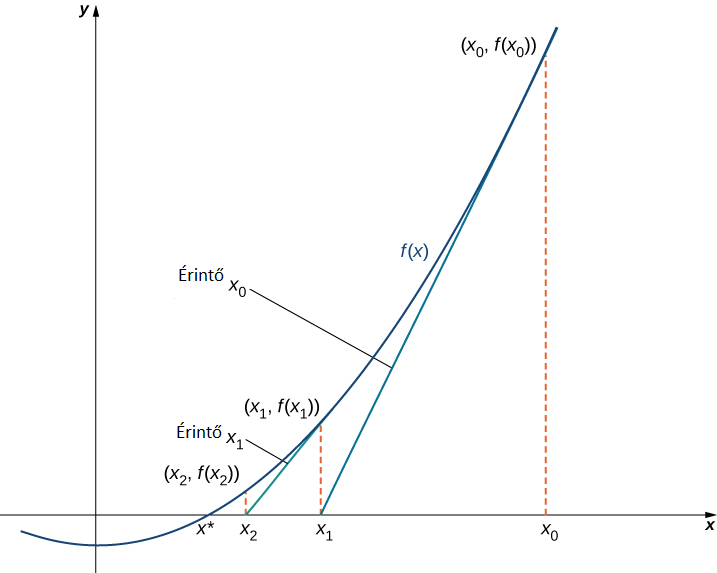
\includegraphics[width=0.5\linewidth]{img/newton_pelda.png}
		\caption{A Newton-módszer alapötlete.}
		\label{fig:newton_pelda}
	\end{figure}

	\noindent Az ábrán a legszélső, $x_{0}$ pontból indulunk, felvesszük a függvény ehhez a ponthoz tartozó
	érintőjét, majd ennek az érintőnek a gyöke lesz a következő pont, és így tovább.\\

    \noindent \textbf{Definíció.} Legyen $f: [a, b]\rightarrow \mathbb{R},\ f \in D[a, b]$, vagyis az $f$ differenciálható az intervallumon, továbbá $f'(x) \neq 0,\ \forall x \in [a, b]$. \\

    \noindent Ekkor az
    \[
        \mybox{
        $x_{n+1} = x_{n} - \ddfrac{f(x_{n})}{f'(x_{n})},\quad n \in \mathbb{N}, \quad x_{0} \in [a, b]$
        }
    \]
    iteráció a Newton-iteráció az $f(x) = 0$ egyenlet megoldására.\\
	
	\noindent A fenti képlet a Newton-iteráció képlete. Megjegyezhető, hogy a fenti módszer is $x_{k+1} = g(x_{k})$
	alakú (fixpontiteráció).\\
	
	\noindent Fontos megemlíteni, hogy $f'(x_{k}) = 0$ esetén nem értelmezhető a módszer. A gyakorlatban $f'(x_{k}) \approx 0$ is probléma.
	Ha $x^{*}$ többszörös gyök, akkor $f'(x^{*}) = 0$, vagyis $x^{*}$ közelében $f'(x_{k})$ egyre jobban közelít $0$-hoz, numerikusan
	instabil.\\
	
	\noindent \textbf{Monoton konvergencia tétele}: Tegyük fel, hogy $f \in \mathcal{C}^{2}([a,b])$ és
    \begin{itemize}
        \item $f'(x) \neq 0,\ f''(x) \neq 0,\ x \in [a, b]$, valamint
        \item $\exists x^{*} \in (a,b) : f(x^{*}) = 0$, és legyen
        \item $x_{0} \in [a, b]$ kezdőpont olyan, hogy $f(x_{0})f''(x_{0}) > 0$ teljesüljön.
    \end{itemize}
	
	\noindent Ekkor az $x_{0}$-ból indított Newton-módszer monoton konvergál $x^{*}$-hoz.\\
	
    \noindent \textbf{Lokális konvergencia tétele}:	Tegyük fel, hogy $f \in \mathcal{C}^{2}([a,b])$ és
    \begin{itemize}
        \item $f'(x) \neq 0,\ x \in [a, b]$, valamint
        \item $\exists x^{*} \in (a,b) : f(x^{*}) = 0$ és legyen
        \item $x_{0} \in [a, b]$ kezdőpont olyan, hogy
        \[
            \big|x_{0} - x^{*}\big| < r := min\Big\{\ddfrac{1}{M},\ |x^{*} - a|,\ |x^{*} - b| \Big\},\ \text{ahol}\
            M = \ddfrac{max_{[a, b]}|f''(x)|}{2 \cdot min_{[a,b]}|f'(x)|}
        \]
    \end{itemize}

    \noindent Ekkor az $x_{0}$-ból indított Newton-iteráció konvergál az $x^{*}$ megoldáshoz, és a konvergencia sebessége p = 2.

	\subsection*{Húrmódszer}
	
	\noindent Továbbra is $f(x) = 0$ megoldása a cél egy adott $[a, b]$ intervallumon.
	Az eljárás lényege a következő. Kezdetben $x_{0} := a, x_{1} := b$, majd meghúzzuk ezen pontok által
	képzett egyenest. Legyen $x_{2}$ a húr gyöke. Ha $f(x_{2}) = 0$, akkor megtaláltuk a gyököt. Ha $f(x_{2}) \not = 0$,
	akkor folytatjuk a keresést az $[x_{0},x_{2}]$ vagy $[x_{2},x_{1}]$ intervallumban. Ha $f(x_{0})f(x_{2}) < 0$, akkor
	$[x_{0},x_{2}]$ intervallumban folytatjuk, ha $f(x_{2}) f(x_{1}) < 0$, akkor $[x_{2}, x_{1}]$ intervallumban. Stb.\\

	\begin{figure}[H]
		\centering
		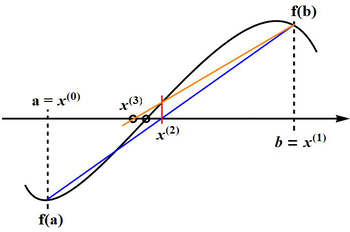
\includegraphics[width=0.5\linewidth]{img/hurmodszer.png}
		\caption{Húr-módszer}
		\label{fig:newton_pelda}
	\end{figure}

	\noindent Általánosan: Legyen $x_{0} := a, x_{1} := b$ és	$f(a)f(b) < 0$. Az $(x_{k},f(x_{k}))$ és $(x_{s},f(x_{s}))$
	pontokon átmenő egyenesekkel közelítjük a függvényt	ahol $x_{s}$-re $f(x_{s})f(x_{k})<0$ és $s$ a legnagyobb ilyen index.
	$x_{k+1}$-et a következőképpen határozhatjuk meg:
	
	\begin{displaymath}
        \mybox{
		$x_{k+1} := x_{k} -
		\ddfrac
		{f(x_{k})}
		{\ddfrac{f(x_{k}) - f(x_{s})}{x_{k}-x_{s}}} =
		x_{k} -
		\ddfrac
		{f(x_{k}) (x_{k} -x_{s}) }
		{f(x_{k}) - f(x_{s})}$
        }
	\end{displaymath}
		
	\noindent \textbf{Tétel}: Legyen $f \in \mathcal{C}^{2}[a,b]$ és
	\begin{enumerate}
		\item	$f(a)f(b)<0$
		\item	$M = \ddfrac{M_{2}}{2m_{1}}$, ahol $0<m_{1} \leq |f'(x)|$ és $f''(x) \leq M_{2} (x \in (a,b))$
		\item	$M(b-a) < 1$
	\end{enumerate}
	
	\noindent Ekkor a húrmódszer konvergens, hibabecslése pedig:
	
	\begin{displaymath}
		|x_{k+1} - x^{*}| \leq \ddfrac{1}{M}(M|x_{0}-x^{*}|)^{k+1}
	\end{displaymath}
	
	\subsection*{Szelőmódszer}
	A szelőmódszer lényege, hogy az $(x_{k},f(x_{k}))$ és $(x_{k-1},f(x_{k-1}))$ pontokon átmenő egyenessel közelítjük
	$f$-et, a kapott egyenes $x$ tengellyel vett metszéspontja $(x_{k+1})$ lesz a következő pont. Ez
	tulajdonképpen a húrmódszer $s := k - 1$-re.
	
	\begin{displaymath}
        \mybox{
		$x_{k+1} :=
		x_{k} -
		\ddfrac
		{f(x_{k}) (x_{k} -x_{k-1}) }
		{f(x_{k}) - f(x_{k-1})}$
        }
	\end{displaymath}
	
	\begin{figure}[H]
		\centering
		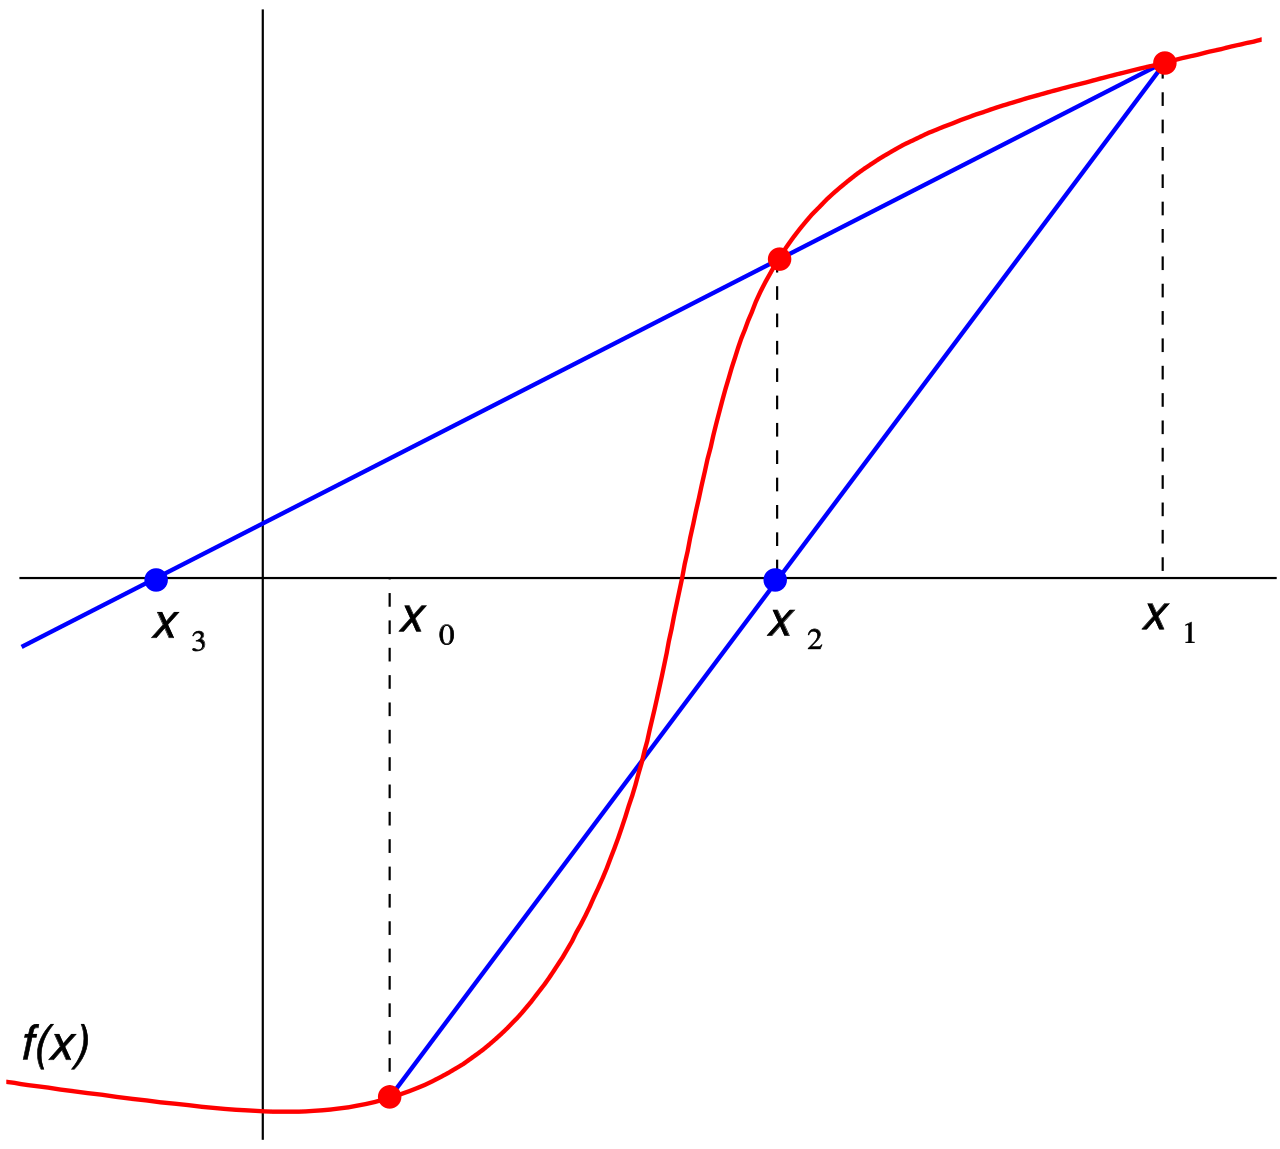
\includegraphics[width=0.5\linewidth]{img/szelomodszer.png}
		\caption{A Newton-módszer alapötlete.}
		\label{fig:newton_pelda}
	\end{figure}

	\noindent \textbf{Tétel}: Ha teljesülnek a Newton-módszer lokális konvergencia tételének feltételei, akkor a szelőmódszer
	konvergens $p = \ddfrac{1+\sqrt{5}}{2}$ rendben, és hibabecslése:
	
	\begin{displaymath}
		|x_{k+1} - x^{*}| \leq M|x_{k}-x^{*}||x_{k-1}-x^{*}|
	\end{displaymath}
	
	\subsubsection*{Többváltozós Newton-módszer}
	
	Most $F(x) = 0$ megoldásait keressük, ahol $F \in \mathbb{R}^{n} \to \mathbb{R}^{n}$. Tekintsük a többváltozós Newton-módszert:
	
	\begin{displaymath}
		\mybox{$x^{(k+1)} := x^{(k)} - [F'(x^{(k)})]^{-1}F(x^{(k)})$}
	\end{displaymath}
	
	\noindent ahol
	
	\begin{displaymath}
		F(x) = \begin{bmatrix}
		f_{1}(x) \\[0.3em]
		f_{2}(x) \\[0.3em]
		\ldots  \\[0.3em]
		f_{n}(x)
		\end{bmatrix}, \quad
		F'(x) = \begin{bmatrix}
		\partial_{1}f_{1}(x) & \partial_{2}f_{1}(x)& ... \\[0.3em]
		\partial_{1}f_{2}(x) & \partial_{2}f_{2}(x)& ... \\[0.3em]
		\ldots & \ldots & \ldots
		\end{bmatrix}
	\end{displaymath}
	
	\noindent Ténylegesen az $F'(x^{(k)}) (x^{(k+1)} - x^{(k)}) = -F(x^{(k)})$ egyenletrendszert oldjuk meg.
	
	\section*{Interpoláció}
	
    \noindent A gyakorlatban sokszor felmerül olyan probléma, hogy egy többségében ismeretlen (csak néhány pontbeli érték ismert) vagy nagyon költségesen kiszámítható függvénnyel kellene egy megadott intervallumon dolgoznunk. Ekkor például azt tehetjük, hogy néhány pontban kiszámítjuk	a függvény értékét, majd keresünk olyan egyszerűbben számítható függvényt, amelyik illeszkedik az adott pontokra. Ezután az intervallum bármely további pontjában az illesztett függvény értékeit használjuk, mint az eredeti függvény értékeinek a közelítéseit. Ilyen egyszerűbben kiszámolható függvények pl. a polinomok (polinom interpoláció).\\
	
    \noindent Példa alkalmazásra: Animáció készítésénél nem szeretnénk minden egyes képkockát saját magunk elkészíteni, hanem csak bizonyos képkockákat, ún. kulcskockákat. A köztes képkockákon az egyes objektumok helyzetét szeretnénk a számítógéppel kiszámíttatani (például szeretnénk, hogy ha egy objektum egyenes vonalú, egyenletes mozgást végezne két adott pozíció között).

	\subsection*{Polinom interpoláció}
	
	\subsubsection*{A polinom interpoláció feladata}
	Legyenek adva $n \in \mathbb{N}$ és az $x_{k} \in \mathbb{R},\ k=0,1,\ldots,n$ különböző számok, az ún. interpolációs alappontok, valamint
	az $f(x_{k}),\ k=0,1,\ldots,n$ számok, az ismert függvényértékek. Keressük azt a legfeljebb $n$-edfokú $p_{n}$ polinomot $(p_{n} \in P_{n})$,
	amelyre:
	
	\begin{displaymath}
		p_{n}(x_{k}) = f(x_{k}) \ \ k=0,1,\ldots,n
	\end{displaymath}
	
	\noindent Azaz a polinom az interpolációs alappontokban a megadott függvényértékeket veszi fel.\\
	
	\noindent \textbf{Tétel}: A fenti interpolációs feladatnak létezik egyértelmű megoldása.\\

    \noindent \textbf{Tétel}: Legyen $n \in N$ és $x_{k} \in R$, $k = 0, 1, \ldots, n$, úgy, hogy $x_{k} \neq x_{l}$, $k \neq l$.\\
    Ekkor létezik olyan $p_{n}(x) = \sum\limits_{i=0}^{n}a_{i}x^{i}$ polinom, hogy
    \[
        p_{n}(x_{k}) = f(x_{k}) \quad k = 0, 1, \ldots, n
    \]
	
	\subsection*{Lagrange-interpoláció}
    Abban az esetben használjuk, ha polinommal szeretnénk közelíteni egy függvényt.  Ennél a módszernél feltesszük, hogy az alappontok páronként különbözők, ami jogos, és ilyenkor adott $x$-re nem mehet át a függvény két $y=f(x)$ értékekhez tartozó ponton. \\
    
    \noindent A módszer egy $n$ alappontból álló sorozat egy $n-1$-edfokú polinommal közelít.\\
    
	\noindent \textbf{Lagrange-alappolinomok}: Adott $n \in \mathbb{N}$ és $x_{k} \in \mathbb{R},\ k=0,1,\ldots,n$ különböző alappontokra, ahol $x_{k} \neq x_{l}$, $k \neq l$,
	a Lagrange-alappolinomokat a következőképpen definiáljuk:
	
	\[
        \mybox{
		$l_{k}(x) = \prod_{\substack{j=0\\j \not = k}}^{n}
		\ddfrac
		{\displaystyle(x-x_{j})}
		{\displaystyle(x_{k}-x_{j})} =
        \ddfrac
        {(x-x_{0})(x-x_{1}) \cdots (x-x_{\textbf{k-1}})(x-x_{\textbf{k+1}}) \cdots (x-x_{n})}
        {(x_{k}-x_{0})(x_{k}-x_{1}) \cdots (x_{k}-x_{\textbf{k-1}})(x_{k}-x_{\textbf{k+1}}) \cdots (x_{k}-x_{n})}$
        }
	\]
	
	\noindent $k=0,1, \ldots, n$ esetén.\\
\newpage	
	\noindent Az alappontok mind $n$-edfokú polinomok, és a következő tulajdonsággal rendelkeznek:
	
	\begin{displaymath}
		l_{k}(x_{j})=\left\{\begin{array}{lr}
		1 & ha \ j=k \\
		0 & ha \ j \not = k
		\end{array}
		\right.
	\end{displaymath}
	
	\noindent \textbf{Tétel}: Az interpolációs feladat megoldása az alábbi polinom, amelyet az interpolációs
	polinom Lagrange-alakjának hívunk:
	
	\begin{displaymath}
		\mybox{$L_{n}(x) = \sum_{k=0}^{n}f(x_{k})l_{k}(x)$}
	\end{displaymath}

	\noindent A továbbiakban jelölje $[a,b]$ az $x_{0}, x_{1}, \ldots, x_{n}$ alappontok által kifeszített intervallumot.\\

%	\noindent \textbf{A Lagrange-interpoláció hibája}: Ha $f \in \mathcal{C}^{n+1}[a,b]$, akkor $\forall x \in [a,b]$ esetén
%	\begin{displaymath}
%		\Big|f(x) - L_{n}(x)\Big| \leq \ddfrac{M_{n+1}}{(n+1)!}\Big|\displaystyle\prod_{i=0}^{n}(x-x_{i})\Big|,\ \text{ahol}\ M_{k} \geq \displaystyle\max_{[a,b]}\Big|f^{(k)}(x)\Big|
%	\end{displaymath}
	
%    \noindent \textbf{Tétel.} Ha $f \in \mathcal{C}^{n+1}([a, b])$, akkor
%    \[
%        \forall x \in [a, b] \quad \exists \xi_{x} \in (a, b) : f(x) - L_{n}(x) = \ddfrac{f^{(n+1)}(\xi_{x})}{(n+1)!}\Omega_{n}(x)
%    \]
%    ahol $\Omega_{n}(x) = (x - x_{0})(x - x_{1})\ldots(x-x_{n})$,
%    továbbá
%    \[
%        \forall x \in [a, b] : \Big|f(x) - L_{n}(x)\Big| \leq \ddfrac{M_{n+1}}{(n+1)!}\Big|\Omega_{n}(x)\Big|
%    \]
%    ahol
%    \[
%        M_{k} \geq \Vert f^{(k)} \Vert_{\infty} = \max\limits_{[a,b]}\Big|f^{(k)(x)}\Big|
%    \]

	\noindent \textbf{Tétel.} Legyen $f \in \mathcal{C}^{\infty}([a,b])$ és legyen adva egy $[a,b]$ intervallumbeli
	alappontrendszerek sorozata: $x_{k}^{n}$, $k=0,1,\ldots,n$, $n=0,1,2,\ldots$. \\

    \noindent Legyen $L_{n}$ az $x_{0}^{n},\ x_{1}^{n},\ \ldots,\ x_{n}^{n}$ alappontrendszerre illesztett Lagrange-interpolációs polinom ($n=0,1,2,\ldots$).\\

    \noindent Ha $\exists M > 0$ úgy, hogy
    \[
	   \forall n \in \mathbb{N} : M_{n} \leq M^{n} \qquad \text{(lásd előző tétel)}
    \]
    akkor az $L_{n}$ sorozat egyenletesen konvergál az $f$ függvényhez.\\

%	\noindent \textbf{Marcinkiewicz tétele}: Minden $f \in \mathcal{C}[a,b]$ esetén létezik a fenti módon definiált alappontrendszer
%	úgy, hogy $\Vert f - L_{n}\Vert_{\infty} \to 0$.\\
	
%	\noindent \textbf{Faber tétele}: Minden a fenti módon definiált alappontrendszer esetén van olyan $f \in \mathcal{C}[a,b]$ függvény,
%	hogy $\Vert f - L_{n}\Vert_{\infty} \not \to 0$.\\

    \noindent A Lagrange-interpoláció hátránya, hogy új alappont hozzávételével az összes számítást újra el kell végezni. Ezt kiküszöbölendő érdemesebb $L_n$-t a következő alakban keresni:
    \[
        N_{n}(x) := A_{0} + A_{1}(x-x_0) + \ldots + A_{n}(x-x_0)\ldots(x-x_{n-1})
    \]

    \noindent Az együtthatók kiszámításához vezetjük be az úgynevezett osztott differenciákat.\\

    {\footnotesize \noindent {\color{blue} \faLightbulbO\ $\triangleright$ } }
    {\footnotesize
    \noindent Ha egy konvergens interpolációt veszünk, akkor felmerül a kérdés, hogy hogyan számítsuk ki egyre magasabb fokszámú interpolációs polinomot azért, hogy növeljük a pontosságot. Viszont a Lagrange-féle interpolációs polinomot minden lépésben újra kellene számolnunk, hiszen az új polinom hozzávételekor minden alappolinom megváltozik. Emiatt olyan előállításra van szükség, amelyik lehetővé teszi, hogy az előzőleg kiszámolt polinomot felhasználhassuk. Az alábbiakban a Newton-féle alakot tárgyaljuk, ami megoldja ezt a problémát: a polinomoknak egy rekurzív előállítását adja. Ehhez először szükség van az osztott differenciák fogalmára.
    $\triangleleft$ \faLightbulbO}\\

	\noindent \textbf{Osztott differencia}: Legyenek adva az $x_{0}, \ldots, x_{n}$ különböző alappontok.
	Az $f:[a,b] \to \mathbb{R}$ függvénynek a megadott alappontrendszerre vonatkozó elsőrendű osztott differenciái, ahol $i = 1,\ \ldots, n$
	\[
		f[x_{i-1},x_{i}] = \ddfrac{f(x_{i})-f(x_{i-1})}{x_{i} - x_{i-1}}
	\]
	$n-1$ darab másodrendű osztott differencia, ahol $i = 2,\ \ldots, n$
	\[
		f[x_{i-2},x_{i-1},x_{i}] = \ddfrac{f[x_{i-1}, x_i] - f[x_{i-2}, x_i]}{x_i - x_{i-2}}
	\]
    ezt általánosítva a $k$-ad rendű osztott differencia $i = k,\ \ldots, n$ esetén
	\[
		\mybox{$f[x_{i-k},x_{i-k+1},\ldots,x_{i}] = \ddfrac{f[x_{i-k+1}, \ldots, x_i] - f[x_{i-k}, \ldots, x_{i-1}]}{x_i - x_{i-k}}$}
	\]

	\noindent Látható, hogy a $k$-adrendű osztott differencia $k+1$ alappontra támaszkodik.\\

	\noindent Ha adott egy interpoláció alappontrendszer függvényértékekkel, akkor a hozzá tartozó osztott differenciákat az
	alábbi táblázat szerint érdemes elrendezni, és ez az elrendezés egyúttal a kiszámolást is segíti (k+1 pont esetén).

	\begin{table}[H]
		\begin{tabular}{llllllll}
			$x_{0}$ & $f(x_{0})$ &  &  &  &  & & \\
             & & $f[x_{0},x_{1}]$ & & & & & \\
			$x_{1}$ & $f(x_{1})$ & & $f[x_0, x_1, x_2]$ &  &  & & \\
            & & $f[x_{1},x_{2}]$ & & & & & \\
			$x_{2}$ & $ f(x_{2})$ & & & & & &\\
			\vdots & \vdots & \vdots & & & $\cdots$ & &\\
			 & & & & & & $f[x_{0}, x_{1}, \cdots, x_{n}]$ &\\
			\vdots & \vdots & \vdots & & & $\cdots$ & &\\
			$x_{n-1}$ & $f(x_{n-1})$ & & $f[x_{n-2},x_{n-1},x_n]$ & & & &\\
            & &  $f[x_{n-1},x_{n}]$ & & & & & \\
			$x_{n} $ & $f(x_{n})$ & & & & \\
		\end{tabular}
	\end{table}
	\noindent \textbf{Állítás.} (Newton-interpolációs formula). A Lagrange-interpolációs polinom megadható a következő formában:
	\begin{displaymath}
		\mybox{$N_{n}(x) = \sum\limits_{k=0}^{n}f[x_{0}, \ldots, x_{k}] \prod\limits_{j=0}^{k-1}(x - x_{j})$}
	\end{displaymath}

    \noindent Észrevehető, hogy érdemesebb a Newton-interpolációs eljárást alkalmazni, hiszen $N_n$-t rekurzívan is ki tudjuk fejezni az	
    \[
        N_{n}(x) = N_{n-1} + f[x_{0}, \ldots, x_{n}](x-x_{0})\ldots(x-x_{n-1})
    \]
    képlet segítségével, így új alappont hozzávételével gyorsabban tudunk interpolációs polinomot számolni.\\

	\subsection*{Hermite-interpoláció}
	Az előbbi interpolációs feladatot a következőképpen általánosíthatjuk. \\

    \noindent Legyenek adva az egyes alappontokban a függvényértékek mellett a függvény derivált értékei is valamely rendig bezárólag. Ekkor olyan polinomot keresünk, amelyik deriváltjaival együtt
	illeszkedik a megadott értékekre, vagyis:\\
	
	\noindent Legyenek adva $m_{0},\ m_{1},\ldots,\ m_{n} \in \mathbb{N}$ és az $x_{j} \in \mathbb{R},\ j=0, 1, \ldots, n$ interpolációs
	alappontok, valamint az $f^{(k)}(x_{j}) \ \ k=0, 1, \ldots, m_{j}-1,\ j=0, 1, \ldots, n$ függvény- és derivált értékek. \\
    Legyen $m = \displaystyle\sum_{j=0}^{n}m_{j}$. Keressük azt a legfeljebb ($m-1$)-edfokú $p_{m-1}$ polinomot, melyre:\\
	
	\[
		\mybox{$p^{(k)}_{m-1}(x_{j}) = f^{(k)}(x_{j}) \qquad (k=0,1,\ldots,m_{j}-1, \ \ \ j=0, 1, \ldots, n)$}
	\]
	
    \noindent \textbf{Definíció.} Az így nyert $p$-t Hermite-interpolációs polinomnak nevezzük és $H_{m}$-mel jelöljük.\\

	\noindent \textbf{Tétel}: A Hermite-féle interpolációs polinom egyértelműen létezik.\\

	\noindent \textbf{Megjegyzések}: Legyen $j=0, 1, \ldots, n$
	\begin{enumerate}
		\item Ha $m_{j}=1$, akkor m = n + 1. Mindegyik $x_{j}$-hez csak az $f_{j}$ érték tartozik. (Lagrange-interpoláció).
		\item Ha $m_{j}=2$. Mindegyik $x_{j}$-hez az $f_{j}$ érték és az $f_{j}^{'}$ derivált érték tartozik. (Hermite-Fejér-féle interpoláció). A keresett polinom pedig legfeljebb ($2n+1$)-edfokú.
	\end{enumerate}
	
	\noindent \textbf{A Hermite interpolációs polinom előállítása\\}

    \noindent Könnyen felírható a Newton-féle formában. Csak annyit
	kell tennünk, hogy kiindulunk az alappontok és a függvényértékek táblázatával és legyártjuk az osztott differenciák
	táblázatát. Az az egyetlen különbség most, hogy az $x_{j}$ alappontot $m_{j}$-szer soroljuk fel.\\

	\noindent Ha $x_{k}$ $j$-szer szerepel:
	\begin{displaymath}
		f[x_{k}, \ldots x_{k}] = \ddfrac{f^{(j)}(x_{k})}{j!}
	\end{displaymath}
	
	\noindent \textbf{Tétel.} (Hermite-interpoláció hibája): \\
    Legyen $\sum\limits_{j=0}^{n}m_{j}$. Ha az $f$ függvény $m$-szer folytonosan differenciálható, akkor
	\begin{displaymath}
		\forall x \in [a,b] \quad \exists \xi \in (a, b): f(x) - H_{m-1}(x) = \ddfrac{f^{(m)}(\xi)}{m!}\Omega_{m}
	\end{displaymath}
	
	\noindent ahol $\Omega_{m}(x) = (x-x_{0})^{m_{0}}(x-x_{1})^{m_{1}}\ldots(x-x_{n})^{m_{n}} = \prod\limits_{i=0}^{n}(x - x_{i})^{m_{i}}$

	\subsection*{Spline-interpoláció}
	
    \noindent A klasszikus interpoláció magas fokszámra nem előnyös alkalmazni. Sok esetben előnyösebb a szakaszonként (alacsony) adott fokszámú interpoláció (spline interpoláció) alkalmazása.\\

    {\footnotesize \noindent {\color{blue} \faLightbulbO\ $\triangleright$ } }
    {\footnotesize
    Bizonyos esetekben probléma lehet a Lagrange-interpolációval, ahol a polinom fokszáma nő az alappontok számával. Ennek következményeként indokolatlanul nagy hullámzások jelennek meg a polinom grafikus képében, két egymást követő pont között. Ez annak tudható be, hogy az eredeti alappontokat szolgáltató $f(x)$ függvény nem polinomiális, és egy közelítő polinom csak úgy tud eleget tenni a feltételeknek, hogy közben lokális minimum és maximum helyeken halad át. Erre nyújt megoldást a spline interpoláció.\\

    \noindent A lényeg, hogy a kicsi fokszámú polinomokból rakjuk össze a közelítő polinomot, mégpedig úgy, hogy először keresünk egy polinomot az első két alappontra, majd a második és harmadik alappontra (és így tovább), de mindezt úgy tesszük, hogy közben figyelünk az illeszkedési pontokban a derivált értékekre (ezzel biztosítva a görbék tökéletes illeszkedését, mivel a spline-ok akkor illeszkednek szépen, ha az alappontokban nem csak az első, hanem a második derivált értéke is megegyezik). \\

    \noindent Létezik elsőfokú, másodfokú, harmadfokú és néhány magasabb fokszámú spline, de gyakorlatban a harmadfokú (cubic) spline-ok a legelterjedtebbek, mert amikor már megvan egy szakaszon a közelítés, és oda akarunk csatlakoztatni egy következő spline-t, akkor van két adatponton érték, illetve a csatlakozási ponton az első és második derivált. Ez négy feltétel, amire egy harmadfokú polinomot lehet illeszteni. $\triangleleft$ \faLightbulbO}\\
\newpage
    \noindent \textbf{$l$-edfokú spline\\}

    \noindent Legyen $\Omega_{n} := [a = x_0 < \ldots < x_n < b]$ felosztás, ahol $l_k := [x_{k-1}, x_k]$ részintervallum ($k = 1, \ldots, n$). Az $\mathbf{S}_{\ell}:[a,b] \to \mathbb{R}$ függvényt egy $\ell$-edfokú spline-nak nevezzük, ha:
	
	\begin{enumerate}
        \item ${\mathbf{S}_{\ell}}_{\big|l_k} \in P_{\ell} \quad (k = 1, \ldots, n)$
		\item $\mathbf{S} \in \mathcal{C}^{\ell-1}[a,b] \quad $ (a teljes intervallumon $(l-1)$-szer folytonosan derviálható)
	\end{enumerate}
\begin{comment}
    \noindent \textbf{Köbös interpolációs spline\\}

    \noindent Legyen $a = x_0 < \ldots < x_n < b$ egy felosztás és $f \in \mathcal{C}[a,b]$ adott és $f(x_i) = y_i \quad (i = 0, \ldots, n)$. Az $f$ függvényt interpoláló köbös $\mathbf{S}(x)$ spline-t a következő módon definiáljuk:
    \begin{itemize}
      \item $S$ szakaszonként harmadfokú polinom, $\mathbf{S}_i(x) := \mathbf{S}_{\big|{[x_i, x_{i+1}]}} \quad (i = 0, \ldots, n-1)$
      \item $\mathbf{S}_i(x) = y_i$ (tehát S interpolálja $f$-et)
      \item $\mathbf{S}_i(x_{i+1}) = \mathbf{S}_{i+1}(x_{i+1}) \quad (i = 1, \ldots, n-2)$ (folytonosan csatlakoznak)
      \item $\mathbf{S}'_i(x_{i+1}) = \mathbf{S}'_{i+1}(x_{i+1}) \quad (i = 1, \ldots, n-2)$ ($\mathbf{S}$-nek nincsenek sarkai)
      \item $\mathbf{S}''_i(x_{i+1}) = \mathbf{S}''_{i+1}(x_{i+1}) \quad (i = 1, \ldots, n-2)$ (görbületek egyenlősége)
      \item Továbbá teljesül még valamelyik a következő peremfeltételek közül
      \begin{itemize}
        \item $\mathbf{S}''(a) = \mathbf{S}''(b) = 0$ (természetes peremfeltételek)
        \item $\mathbf{S}'(a) = f'(a), \quad \mathbf{S}'(b) = f'(n)$ (Hermite feltételek)
        \item $\mathbf{S}'(a) = S'(b), \quad \mathbf{S}''(a) = S''(b)$ (Periodikus feltételek)
      \end{itemize}
    \end{itemize}
\end{comment}

    \noindent Részintervallumonkénti polinomok együtthatóinak megkeresése:

    \[
        p_{k}(x) = \sum\limits_{j=0}^{\ell}a^{(k)}_{j} \cdot (x - x_{k-1})^{k} \quad (x \in l_{k})
    \]

	\noindent \textbf{Spline megadás intervallumonként\\}

%    \noindent Legyenek adottak $x_{k},\ f(x_{k})$ értékek $k=0, \ldots, n$-re és $\ell \in \mathbb{N}$.
%	Keressük azt az $\mathbf{S} \in \mathbf{S}_{\ell}(\Omega_{n})$ spline-t, amelyre $\mathbf{S}(x_{k}) = f(x_{k})$.\\

    \noindent \textbf{$\ell = 1$ elsőfokú spline megadása\\}

    \noindent A legegyszerűbb eset a szakaszonként lineáris spline interpoláció. Ebben az esetben az interpolációban szakaszonként egy egyenessel kötünk össze két egymás mellett lévő pontot.

    \[
        p_{k}(x) = a_1^{(k)}(x - x_{k-1}) + a_{0}^{(k)} \quad (x \in l_{k})
    \]

    \noindent A megoldáshoz írjuk fel az interpolációs feltételeket az $l_k$ részintervallum két szélére.

    \begin{center}
        $p_{k}(x_{k-1}) = a_{0}^{(k)} = f(x_{k-1})$\\
        $p_{k}(x_{k}) = a_1^{(k)}(x_{k} - x_{k-1}) + a_{0}^{(k)} = f(x_{k})$\\
        $\Downarrow$\\
        \mybox{$a_{1}^{(k)} = \ddfrac{f(x_{k}) - f(x_{k-1})}{x_{k} - x_{k-1}} = f[x_{k-1}, x_{k}]$}
    \end{center}

    \noindent Az interpolációs feltételből a folytonosság azonnal következik.\\

    \noindent \textbf{$\ell = 2$ másodfokú (kvadratikus) spline megadása\\}
    \[
        \mybox{$p_{k}(x) = a_2^{(k)}(x - x_{k-1})^2 + a_1^{(k)}(x - x_{k-1}) + a_{0}^{(k)} \quad (x \in l_{k})$}
    \]

    \begin{itemize}
        \item Az ismeretlenek száma: 3n.
        \item A feltételek száma:
        \begin{itemize}
            \item interpolációs feltétel minden részintervallum két szélére: \textbf{2n} feltétel\\
            (n intervallumra felosztva, intervallumonként 2 végponttal)
        \end{itemize}
        \item minden belső osztópontra a folytonos differenciálhatóság: \textbf{n-1} feltétel
    \end{itemize}

    \noindent Összesen $2n + n-1 = \textbf{3n-1}$ feltétel van, vagyis az egyértelműséghez hiányzik egy feltétel.\\
    Ezt peremfeltételként szokás megadni:
    \[
        \mathbf{S}'(a) = f'(a), \quad \mathbf{S}'(b) = f'(n)\ \text{(Hermite feltételek)}
    \]

    \noindent A feladat szétbontható $n$ db Hermite-interpolációs feladattá.\\
\newpage
    \noindent \textbf{$\ell = 3$ harmadfokú (köbös) spline megadása\\}
    \[
        \mybox{$p_{k}(x) = a_3^{(k)}(x - x_{k-1})^3 + a_2^{(k)}(x - x_{k-1})^2 + a_1^{(k)}(x - x_{k-1}) + a_{0}^{(k)} \quad (x \in l_{k})$}
    \]

    \begin{itemize}
        \item Az ismeretlenek száma: 4n.
        \begin{itemize}
            \item interpolációs feltétel minden részintervallum két szélére: \textbf{2n} feltétel\\
            (n intervallumra felosztva, intervallumonként 2 végponttal)
        \end{itemize}
        \item minden belső osztópontra $\mathbf{S}'_{3} \in \mathcal{C}$: \textbf{n-1} feltétel
        \item minden belső osztópontra $\mathbf{S}''_{3} \in \mathcal{C}$: \textbf{n-1} feltétel
    \end{itemize}

    \noindent Összesen $2n + n-1 + n-1 = \textbf{4n-2}$ feltétel van, vagyis az egyértelműséghez hiányzik két feltétel. Ezt peremfeltételként szokás megadni:
    \[
        \mathbf{S}'(a) = f'(a), \quad \mathbf{S}'(b) = f'(n)\ \text{(Hermite feltételek)}
    \]

    \[
        \mathbf{S}''(a) = \mathbf{S}''(b) = 0\ \text{(Természetes peremfeltételek)}
    \]

    \noindent Csak periodikus függvények közelítése esetén, ha $[a, b]$ a periódus többszöröse.\\
    Ekkor $f(a) = f(b)$ és a két hiányzó feltétel:
    \[
        \mathbf{S}'(a) = S'(b), \text{és} \quad \mathbf{S}''(a) = S''(b)\ \text{(Periodikus feltételek)}
    \]

    \subsection*{B-Spline\\}
	
	\noindent \textbf{Definíció.} (Függvény tartója): Az $f: \mathbb{R} \rightarrow \mathbb{R}$ \emph{\textbf{függvény tartója}} a következő valós számhalmaz:
    \[
        supp(f) := \overline{\left\{x \in \mathbb{R}: f(x) \not = 0 \right\}}
    \]

	\noindent \textbf{Definíció.} (Alappontrendszer): $\Omega_{\infty} := \left\{\ldots, x_{-n}, \ldots, \ldots, x_{-1}, x_{0}, x_{1}, \ldots, x_{n}, \ldots\right\}$\\
	
	\noindent $\mathbf{S}_{l}(\Omega_{\infty})$ az $\Omega_{n}$ alappontrendszeren értelmezett $l$-edfokú spline-ok halmaza.\\

	\noindent \textbf{B-spline}: A $B_{l,k} \in \mathbf{S}_{l}(\Omega_{\infty}),\ (k \in \mathbb{Z})$ $l$-edfokú spline függvények rendszerét B-spline függvényeknek
	nevezzük, ha az alábbi feltételek teljesülnek:
	\begin{enumerate}
		\item	$B_{l,k}(x) \geq 0$
		\item	$supp(B_{l,k}) = [x_{k},x_{k+l+1}]$, azaz a tartója minimális
		\item	$\displaystyle\sum_{k \in \mathbb{Z}}B_{l,k}(x) \equiv 1 \quad (\forall x \in \mathbb{R})$
	\end{enumerate}
	
	\section*{Legkisebb négyzetek módszere}
	
	Gyakorlati feladatok során adódik a következő probléma. Egy elsőfokú függvényt mérünk bizonyos pontokban, de
	a mérési hibák miatt ezek nem lesznek egy egyenesen. Ekkor olyan egyenest keresünk, amelyik az alábbi
	értelemben legjobban illeszkedik a megadott mérési ponthalmazra.
	
    \paragraph*{Egyenes eset}

	\noindent Legyenek adva az $(x_{i},y_{i}),\ i=1,2,\ldots,n$ mérési pontok.\\
    \noindent Keressük azt a $p_{1}(x) = a + bx$ legfeljebb elsőfokú polinomot, amelyre a következő kifejezés minimális.
	
	\begin{displaymath}
        \mybox{
		$\displaystyle\sum_{i=1}^{n}(y_{i}-p_{1}(x_{i}))^{2} =
		\displaystyle\sum_{i=1}^{n}(y_{i}-a-bx_{i})^{2}$
        }
	\end{displaymath}

	\noindent Ez azt jelenti, hogy azt az egyenes keressük, amelyre a függvényértékek hibáinak
	négyzetösszege minimális.
	
    \paragraph*{Polinom eset\\}

	\noindent Adottak az $n, N \in \mathbb{N}$, ahol $n \ll N$ és $(x_{i},y_{i}),\ i= 1,2,\ldots,n$ mérési pontok, ahol az $x_{i}$
	alappontok különbözők.\\
    \noindent Keressük azt a $p_{n}(x) = a_{0} + a_{1}x + \ldots + a_{n}x^{n} = \sum\limits_{i=0}^{n}a_{j}x^{j}$ legfeljebb $n$-edfokú polinomot, melyre a következő kifejezés minimális.

	\begin{displaymath}
	   \mybox{$\displaystyle\sum_{i=1}^{m}(y_{i}-p_{n}(x_{i}))^{2}$}
	\end{displaymath}

    {\footnotesize
    \noindent \textbf{Definíció}: Az $m \times n$-es $A$ mátrix transzponáltján azt az $A^{T}$-vel jelölt $n \times m$-es mátrixot értjük, amelyet az $A$ sorainak és oszlopainak felcserélésével kapunk. Azaz
    \[
        A^{T} = [a_{ij}]^{T} = [a_{ji}]
    \]
    }
	\noindent A feladat megoldásához tekintsük annak egy átfogalmazását.\\
	
	\noindent Vegyük a $p_{n}(x_{i}) = y_{i}, (i=1,2,...,m)$ egyenletrendszert. Ez a rendszer az ismeretlen $a_{i}$ együtthatókra nézve
	lineáris, mégpedig túlhatározott, amelynek az $A$ mátrixa egy téglalap alakú Vandermonde-mátrix $A \in \mathbb{R}^{m \times (n+1)}$,
	a $b \in \mathbb{R}^{m}$ jobb oldali vektorra pedig a függvényértékekből adódik:
	
{\small
	\begin{displaymath}
	\begin{bmatrix}
	1 & x_{1} & x_{1}^{2} & ... & x_{1}^{n} \\[0.3em]
	1 & x_{2} & x_{2}^{2} & ... & x_{2}^{n} \\[0.3em]
	1 & x_{3} & x_{3}^{2} & ... & x_{3}^{n} \\[0.3em]
	\rotatebox[origin=c]{90}{...} & \rotatebox[origin=c]{90}{...} &\rotatebox[origin=c]{90}{...} & \rotatebox[origin=c]{90}{...} & \rotatebox[origin=c]{90}{...} \\[0.3em]
	1 & x_{m} & x_{m}^{2} & ... & x_{m}^{n} \\[0.3em]
	\end{bmatrix}
	\begin{bmatrix}
	a_{0} \\[0.3em]
	a_{1} \\[0.3em]
	a_{2} \\[0.3em]
	\rotatebox[origin=c]{90}{...} \\[0.3em]
	a_{n}
	\end{bmatrix}
	=
	\begin{bmatrix}
	y_{0} \\[0.3em]
	y_{1} \\[0.3em]
	y_{2} \\[0.3em]
	\rotatebox[origin=c]{90}{...} \\[0.3em]
	y_{m}
	\end{bmatrix}
	\end{displaymath}
}	
	\noindent Ezen jelölésekkel a minimalizálandó kifejezés $\Vert Az - b \Vert_{2}^{2}$, ahol $z = [a_{0},a_{1}, ..., a_{n}]^{T}$
	a keresett együtthatók vektorra. A feladat megoldását a Gauss-féle normálegyenletek adják:
	
	\begin{displaymath}
		A^{T}Az = A^{T}b
	\end{displaymath}
	
	\noindent A fenti lineáris egyenletrendszert kell megoldani $z$-re.\\
	
	\noindent \textbf{n=1 eset}: Ekkor a feladatot gyakran lineáris regressziónak is hívjuk. Ebben az esetben
	\begin{displaymath}
		A^{T}A = \begin{bmatrix}
		m & \sum\limits_{i=1}^{m} x_{i} \\[0.3em]
		\sum\limits_{i=1}^{m} x_{i} & \sum_{i=1}^{m} x_{i}^{2}
		\end{bmatrix} \ ,
		A^{T}b = \begin{bmatrix}
		\sum\limits_{i=1}^{m} y_{i} \\[0.3em]
		\sum\limits_{i=1}^{m} x_{i}y_ {i}
		\end{bmatrix} \ ,
		z = \begin{bmatrix}
		b \\[0.3em]
		a
		\end{bmatrix}
	\end{displaymath}
\newpage
    \subsection*{Kiegészítés}
    \small
    \paragraph*{Elégséges feltétel a konvergenciára (lineáris egyenletrendszer)}

    \noindent Tekintsük az $\underline{x} = B\underline{x} + \underline{r}$ egyenletet, ahol $\Vert B \Vert < 1$ valamely indukált vagy illeszkedő normában.\\

    \noindent Ekkor
    \begin{itemize}
        \item $\exists! x^{*} \in \mathbb{R}^{n} : x^{*} = B\underline{x}^{*} + \underline{r}$
        \item $\forall \underline{x}^{(0)} \in \mathbb{R}^{n}$ kezdőérték esetén, az $\underline{x}^{(k+1)} = B\underline{x}^{(k)} + \underline{r}$ rekurzióval definiált sorozat konvergens, és a határértéke az $x^{*}$ lesz, vagyis
            \[
                \lim\limits_{k \to \infty} \underline{x}^{(k)} = \underline{x}^{*}
            \]
        \item teljesül az alábbi hibabecslés is:
        \[
            \Vert \underline{x}^{(k)} - \underline{x}^{*} \Vert \leq \ddfrac{\Vert B \Vert^{k}}{1 - \Vert B \Vert}\Vert \underline{x}^{(1)} - \underline{x}^{(0)} \Vert
        \]
    \end{itemize}
\centerline{\rule{17cm}{0.4pt}}
    \noindent Az $L$ mátrix \emph{alsó háromszögmátrix}, az $A$ mátrix szigorú alsó része, vagyis
    \[
        l_{i,j} = a_{i,j},\ \text{ha}\ i > j,\ \text{különben}\ 0,
        \left(
          \begin{array}{cccc}
            0 & 0 & \cdots & 0 \\
            \textbf{x} & 0 & \ddots & \vdots \\
            \vdots & \ddots & \ddots & \vdots \\
            \textbf{x} & \cdots & \textbf{x} & 0 \\
          \end{array}
        \right)
    \]
    az $U$ \emph{felső háromszögmátrix}, az $A$ mátrix szigorú felső része, vagyis
    \[
        u_{i,j} = a_{i, j},\ \text{ha}\ i < j,\ \text{különben}\ 0,
        \left(
          \begin{array}{cccc}
            0 & \textbf{x} & \cdots & \textbf{x} \\
            0 & 0 & \ddots & \vdots \\
            \vdots & \ddots & \ddots & \textbf{x} \\
            0 & \cdots & 0 & 0 \\
          \end{array}
        \right)
    \]
    a $D$ pedig \emph{invertálható diagonális mátrix} az $A$ mátrix diagonális része, vagyis
    \[
        d_{i, j} = a_{i, j},\ \text{ha}\ i = j,\ \text{különben}\ 0.
        \left(
          \begin{array}{cccc}
            \textbf{x} & 0 & \cdots & 0 \\
            0 & \textbf{x} & \ddots & \vdots \\
            \vdots & \ddots & \ddots & \vdots \\
            0 & \cdots & 0 & \textbf{x}
          \end{array}
        \right)
    \]
\centerline{\rule{17cm}{0.4pt}}
    \noindent A Jacobi-iteráció kanonikus alakját a következő átalakításokkal kaphatjuk meg:
    \begin{center}
        $\underline{x}^{(k+1)} = -D^{-1}(L + U)\underline{x}^{(k)} + D^{-1}\underline{b}$ \\
        $D\underline{x}^{(k+1)} + (L + U)\underline{x}^{(k)} = \underline{b}$ \\
        $D(\underline{x}^{(k+1)} - \underline{x}^{(k)}) + (L + U)\underline{x}^{(k)} + D\underline{x}^{(k)} = \underline{b}$ \\
        $D(\underline{x}^{(k+1)} - \underline{x}^{(k)}) + \underbrace{(L + U + D)}_{=A}\underline{x}^{(k)} = \underline{b}$ \\
        $D(\underline{x}^{(k+1)} - \underline{x}^{(k)}) + A\underline{x}^{(k)} = \underline{b}$
    \end{center}

    \noindent \textbf{Állítás}. Ha a Jacobi iteráció által előállított ($\underline{x}^{(k)}$) vektorsorozat konvergens, azaz létezik $\underline{x}^{*}$, melyre $\lim\limits_{k \to \infty}\underline{x}^{(k)} = \underline{x}^{*}$, akkor $\underline{x}^{*}$ megoldása az $A\underline{x} = \underline{b}$ egyenletrendszernek.\\

    \noindent \textbf{Bizonyítás}. A Jacobi-iteráció kanonikus képletében térjünk át limeszre, és felhasználva, hogy $\lim\lambda x = \lambda \lim x\ \text{és} \lim(A + B) = \lim A + \lim B$
    \[
        \lim\limits_{k \to \infty}\Big[D(\underline{x}^{(k+1)} - \underline{x}^{(k)}) + A\underline{x}^{(k)}\Big] = D \lim\limits_{k \to \infty}(\underbrace{\underline{x}^{(k+1)} - \underline{x}^{(k)}}_{\to \underline{x}^{*} - \underline{x}^{*} = 0}) + A \lim\limits_{k \to \infty}\underbrace{\underline{x}^{(k)}}_{\to \underline{x}^{*}} = A\underline{x}^{*} = \underline{b}
    \]
    \noindent Felhasználva, hogy $\lim\lambda x = \lambda \lim x\ \text{és} \lim(A + B) = \lim A + \lim B$.

    \noindent Ha az $Ax = b$ lineáris egyenletrendszer mátrixa szigorúan diagonálisan domináns
    \[
        ||B_{J}||_{\infty} = ||-D^{-1}(L+U)||_{\infty} = \max_{1 \leq k \leq n} \sum_{\substack{i=1\\ i \not = k}}^{n} \ddfrac{|a_{i,k}|}{|a_{i,i}|} = \max_{1 \leq k \leq n}\ddfrac{1}{|a_{i,i}|} \sum_{\substack{i=1\\ i \not = i}}^{n} |a_{i,k}| < 1 \qquad \text{(soraira)}
    \]
    \[
        ||B_{J}||_{1} = ||-D^{-1}(L+U)||_{1} = \max_{1 \leq i \leq n} \sum_{\substack{k=1\\ k \not = i}}^{n} \ddfrac{|a_{i,k}|}{|a_{i,i}|} = \max_{1 \leq i \leq n}\ddfrac{1}{|a_{i,i}|} \sum_{\substack{k=1\\ k \not = i}}^{n} |a_{i,k}| < 1 \qquad \text{(oszlopaira)}
    \]
    akkor a Jakobi-iteráció konvergens.\\
\centerline{\rule{17cm}{0.4pt}}
    \noindent Példa Jacobi-iterációra. Tekintsük a következő egyenletrendszert:
    \begin{center}
        $\begin{bmatrix}
            5 & -2 & 1 \\[0.3em]
            0 & 3 & -1 \\[0.3em]
            2 & -1 & 6 \\[0.3em]
        \end{bmatrix}_{A}$\underline{x} =
        $\begin{bmatrix}
            4 \\[0.3em]
            2 \\[0.3em]
            7 \\[0.3em]
        \end{bmatrix}_{b}$
    \end{center}

    \noindent Képezzük a Jacobi iteráció komponensenkénti alakját, majd számoljuk ki az első négy iterációs lépést az $x^{(0)} = \left[0,0,0\right]^{T}$ vektorból kiindulva.
	
    \begin{center}
            $5x_1 -2x_2 + x_3 = 4$ \\
            $3x_2 -x_3 = 2$ \\
            $2x_1 - x_2 + 6x_3 = 7$ \\
            $\downarrow$
    \end{center}
    \begin{center}
            $5x_1 = 4 + 2x_2 - x_3$ \\
            $3x_2 = 2 + x_3 $ \\
            $6x_3 = 7 - 2x_1 + x_2$ \\
            $\downarrow$
    \end{center}

    \begin{center}
            $x_1 = \ddfrac{4}{5} + \ddfrac{2x_2}{5} - \ddfrac{x_3}{5}$ \\
            $x_2 = \ddfrac{2}{3} + \ddfrac{x_3}{3} $ \\
            $x_3 = \ddfrac{7}{6} - \ddfrac{2x_1}{6} + \ddfrac{x_2}{6}$ \\
            $\downarrow$ {\tiny (átrendezés után)}
    \end{center}

    \begin{center}
            $x_1^{(k+1)} = \ddfrac{\textbf{2}}{\textbf{5}} x_2^{(k)} - \ddfrac{\textbf{1}}{\textbf{5}}x_3^{(k)} + \ddfrac{\textbf{4}}{\textbf{5}} $ \\
            $x_2^{(k+1)} = \ddfrac{\textbf{1}}{\textbf{3}}x_3^{(k)} + \ddfrac{\textbf{2}}{\textbf{3}}$ \\
            $x_3^{(k+1)} = - \ddfrac{\textbf{2}}{\textbf{6}}x_1^{(k)} + \ddfrac{\textbf{1}}{\textbf{6}}x_2^{(k)} + \ddfrac{\textbf{7}}{\textbf{6}}$ \\
    \end{center}

    \noindent Írjuk vissza mátrix alakra:

    \begin{center}
        $\begin{bmatrix}
            x_1^{(k+1)} \\[0.3em]
            x_2^{(k+1)} \\[0.3em]
            x_3^{(k+1)} \\[0.3em]
        \end{bmatrix}$ =
        $\begin{bmatrix}
            0 & \ddfrac{\textbf{2}}{\textbf{5}} & -\ddfrac{\textbf{1}}{\textbf{5}} \\[0.3em]
            0 & 0 & \ddfrac{\textbf{1}}{\textbf{3}} \\[0.3em]
            -\ddfrac{\textbf{2}}{\textbf{6}} & \ddfrac{\textbf{1}}{\textbf{6}} & 0 \\[0.3em]
        \end{bmatrix}_{A} \cdot$
        $\begin{bmatrix}
            x_1^{(k)} \\[0.3em]
            x_2^{(k)} \\[0.3em]
            x_3^{(k)} \\[0.3em]
        \end{bmatrix}$+
        $\begin{bmatrix}
            \ddfrac{\textbf{4}}{\textbf{5}} \\[0.3em]
            \ddfrac{\textbf{2}}{\textbf{3}} \\[0.3em]
            \ddfrac{\textbf{7}}{\textbf{6}} \\[0.3em]
        \end{bmatrix}$
    \end{center}

    \noindent A kezdővektor $x^{(0)} = \left[0,0,0\right]^{T}$, így az első négy iterációs lépés a következő.

    \begin{center}
        $x^{(1)}$ =
        $\begin{bmatrix}
            0 & -\ddfrac{2}{5} & \ddfrac{1}{5} \\[0.3em]
            0 & 0 & \ddfrac{1}{3} \\[0.3em]
            -\ddfrac{2}{6} & \ddfrac{1}{6} & 0 \\[0.3em]
        \end{bmatrix}_{A} \cdot$
        $\begin{bmatrix}
            0 \\[0.3em]
            0 \\[0.3em]
            0 \\[0.3em]
        \end{bmatrix}_{x^{(0)}}$+
        $\begin{bmatrix}
            \ddfrac{4}{5} \\[0.3em]
            \ddfrac{2}{3} \\[0.3em]
            \ddfrac{7}{6} \\[0.3em]
        \end{bmatrix}_{b}$=
        $\begin{bmatrix}
            \ddfrac{\textbf{4}}{\textbf{5}} \\[0.3em]
            \ddfrac{\textbf{2}}{\textbf{3}} \\[0.3em]
            \ddfrac{\textbf{7}}{\textbf{6}} \\[0.3em]
        \end{bmatrix}_{x^{(1)}}$
    \end{center}
    \begin{center}
        $x^{(2)}$ =
        $\begin{bmatrix}
            0 & -\ddfrac{2}{5} & \ddfrac{1}{5} \\[0.3em]
            0 & 0 & \ddfrac{1}{3} \\[0.3em]
            -\ddfrac{2}{6} & \ddfrac{1}{6} & 0 \\[0.3em]
        \end{bmatrix}_{A} \cdot$
        $\begin{bmatrix}
            \ddfrac{\textbf{4}}{\textbf{5}} \\[0.3em]
            \ddfrac{\textbf{2}}{\textbf{3}} \\[0.3em]
            \ddfrac{\textbf{7}}{\textbf{6}} \\[0.3em]
        \end{bmatrix}_{x^{(1)}}$+
        $\begin{bmatrix}
            \ddfrac{4}{5} \\[0.3em]
            \ddfrac{2}{3} \\[0.3em]
            \ddfrac{7}{6} \\[0.3em]
        \end{bmatrix}_{b}$=
        $\begin{bmatrix}
            \ddfrac{\textbf{5}}{\textbf{8}} \\[0.3em]
            \ddfrac{\textbf{19}}{\textbf{18}} \\[0.3em]
            \ddfrac{\textbf{91}}{\textbf{90}} \\[0.3em]
        \end{bmatrix}_{x^{(2)}}$
    \end{center}
    \begin{center}
        $x^{(3)}$ =
        $\begin{bmatrix}
            0 & -\ddfrac{2}{5} & \ddfrac{1}{5} \\[0.3em]
            0 & 0 & \ddfrac{1}{3} \\[0.3em]
            -\ddfrac{2}{6} & \ddfrac{1}{6} & 0 \\[0.3em]
        \end{bmatrix}_{A} \cdot$
        $\begin{bmatrix}
            \ddfrac{\textbf{5}}{\textbf{8}} \\[0.3em]
            \ddfrac{\textbf{19}}{\textbf{18}} \\[0.3em]
            \ddfrac{\textbf{91}}{\textbf{90}} \\[0.3em]
        \end{bmatrix}_{x^{(2)}}$+
        $\begin{bmatrix}
            \ddfrac{4}{5} \\[0.3em]
            \ddfrac{2}{3} \\[0.3em]
            \ddfrac{7}{6} \\[0.3em]
        \end{bmatrix}_{b}$=
        $\begin{bmatrix}
            \ddfrac{\textbf{51}}{\textbf{50}} \\[0.3em]
            \ddfrac{\textbf{271}}{\textbf{270}} \\[0.3em]
            \ddfrac{\textbf{115}}{\textbf{108}} \\[0.3em]
        \end{bmatrix}_{x^{(3)}}$
    \end{center}
    \begin{center}
        $x^{(4)}$ =
        $\begin{bmatrix}
            0 & -\ddfrac{2}{5} & \ddfrac{1}{5} \\[0.3em]
            0 & 0 & \ddfrac{1}{3} \\[0.3em]
            -\ddfrac{2}{6} & \ddfrac{1}{6} & 0 \\[0.3em]
        \end{bmatrix}_{A} \cdot$
        $\begin{bmatrix}
            \ddfrac{\textbf{51}}{\textbf{50}} \\[0.3em]
            \ddfrac{\textbf{271}}{\textbf{270}} \\[0.3em]
            \ddfrac{\textbf{115}}{\textbf{108}} \\[0.3em]
        \end{bmatrix}_{x^{(3)}}$+
        $\begin{bmatrix}
            \ddfrac{4}{5} \\[0.3em]
            \ddfrac{2}{3} \\[0.3em]
            \ddfrac{7}{6} \\[0.3em]
        \end{bmatrix}_{b}$=
        $\begin{bmatrix}
            \ddfrac{2669}{2700} \\[0.3em]
            \ddfrac{331}{324} \\[0.3em]
            \ddfrac{8051}{8100} \\[0.3em]
        \end{bmatrix}_{x^{(4)}}$
    \end{center}
    \renewcommand{\arraystretch}{1}
%---
\centerline{\rule{17cm}{0.4pt}}
    \noindent A Gauss-Seidel kanonikus alakját a következő átalakításokkal kaphatjuk meg:
    \begin{center}
        $\underline{x}^{(k+1)} = -(D + L)^{-1}U\underline{x}^{(k)} + (D + L)^{-1}\underline{b}$ \\
        $(D + L)\underline{x}^{(k+1)} + U\underline{x}^{(k)} = \underline{b}$ \\
        $(D + L)\underline{x}^{(k+1)} - (D + L)\underline{x}^{(k)} + U\underline{x}^{(k)} + (D + L)\underline{x}^{(k)} = \underline{b}$ \\
        $(D + L)(\underline{x}^{(k+1)} - {x}^{(k)}) + \underbrace{(U + D + L)}_{=A}\underline{x}^{(k)} = \underline{b}$ \\
        $(D + L)(\underline{x}^{(k+1)} - {x}^{(k)}) + A\underline{x}^{(k)} = \underline{b}$ \\
    \end{center}

    \noindent \textbf{Állítás}. Ha a Gauss-Seidel iteráció által előállított ($\underline{x}^{(k)}$) vektorsorozat konvergens, azaz létezik $\underline{x}^{*}$, melyre $\lim\limits_{k \to \infty}\underline{x}^{(k)} = \underline{x}^{*}$, akkor $\underline{x}^{*}$ megoldása az $A\underline{x} = \underline{b}$ egyenletrendszernek.\\

    \noindent \textbf{Bizonyítás}. A Gauss-Seidel-iteráció kanonikus képletében térjünk át limeszre, és felhasználva, hogy $\lim\lambda x = \lambda \lim x\ \text{és} \lim(A + B) = \lim A + \lim B$.
    \[
        \lim\limits_{k \to \infty}\Big[(D + L)(\underline{x}^{(k+1)} - \underline{x}^{(k)}) + A\underline{x}^{(k)}\Big] = (D + L) \lim\limits_{k \to \infty}(\underbrace{\underline{x}^{(k+1)} - \underline{x}^{(k)}}_{\to \underline{x}^{*} - \underline{x}^{*} = 0}) + A \lim\limits_{k \to \infty}\underbrace{\underline{x}^{(k)}}_{\to \underline{x}^{*}} = A\underline{x}^{*} = \underline{b}
    \]
%---
\centerline{\rule{17cm}{0.4pt}}
    \noindent Példa a Gauss-Seidel iterációra. Tekintsük a következő egyenletrendszert:
    \renewcommand{\arraystretch}{2}
    \begin{center}
        $\begin{bmatrix}
            -5 & -2 & 1 \\[0.3em]
            1 & 3 & -1 \\[0.3em]
            2 & -1 & 6 \\[0.3em]
        \end{bmatrix}$x =
        $\begin{bmatrix}
            1 \\[0.3em]
            1 \\[0.3em]
            1 \\[0.3em]
        \end{bmatrix}$
    \end{center}

    \begin{center}
        $\begin{bmatrix}
            \textbf{-5}_{a_{1,1}} & \textbf{-2}_{a_{1,2}} & \textbf{1}_{a_{1,3}} \\[0.3em]
            \textbf{1}_{a_{2,1}} & \textbf{3}_{a_{2,2}} & \textbf{-1}_{a_{2,3}} \\[0.3em]
            \textbf{2}_{a_{3,1}} & \textbf{-1}_{a_{3,2}} & \textbf{6}_{a_{3,3}} \\[0.3em]
        \end{bmatrix}$x =
        $\begin{bmatrix}
            b_{1}=1 \\[0.3em]
            b_{2}=1 \\[0.3em]
            b_{3}=1 \\[0.3em]
        \end{bmatrix}$
    \end{center}

    \noindent A kezdővektor $x^{(0)} = \left[0,0,0\right]^{T}$, így az első két iterációs lépés a következő.\\
    \renewcommand{\arraystretch}{1}

	$
    x^{(1)}_{1} =
	-\ddfrac{1}{a_{1,1}}
	\Bigg(
	\sum\limits_{j=1}^{0} a_{1,j}x_{j}^{(1)} +
	\sum\limits_{j=2}^{3} a_{1,j}x_{j}^{(0)} -
	b_{1}
	\Bigg)=
	-\ddfrac{1}{-5}
	\Bigg(
	0 +
	a_{1,1}x_{1}^{(0)} + a_{1,3}x_{3}^{(0)} -
	b_{1}
	\Bigg)=\\
	= \ddfrac{1}{5}
	\Bigg(
	-5x_{1}^{(0)} + x_{3}^{(0)} - 1
    \Bigg)=
    -x_{1}^{(0)} + \ddfrac{1}{3}x_{3}^{(0)} - \ddfrac{1}{5}
    =
    -0 + \ddfrac{1}{3} \cdot 0 - \ddfrac{1}{5} = \textbf{-}\ddfrac{\textbf{1}}{\textbf{5}}
    $\\\\

	$
    x^{(1)}_{2} =
	-\ddfrac{1}{a_{2,2}}
	\Bigg(
	\sum\limits_{j=1}^{1} a_{2,j}x_{j}^{(1)} +
	\sum\limits_{j=3}^{3} a_{2,j}x_{j}^{(0)} -
	b_{2}
	\Bigg)=
	-\ddfrac{1}{3}
	\Bigg(
	1 \cdot x_{1}^{(1)} +
	a_{2,3}x_{3}^{(0)} -
	b_{2}
	\Bigg)=\\
	-\ddfrac{1}{3}
	\Bigg(
    -\ddfrac{1}{5} -
	0 -
    1
    \Bigg)=
	-\ddfrac{5}{15}
	\Bigg(
    -\ddfrac{3}{15} -
    \ddfrac{15}{15}
    \Bigg)=
    \ddfrac{90}{225} = \ddfrac{\textbf{2}}{\textbf{5}}
    $

	$
    x^{(1)}_{3} =
	-\ddfrac{1}{a_{3,3}}
	\Bigg(
	\sum\limits_{j=1}^{2} a_{3,j}x_{j}^{(1)} +
	\sum\limits_{j=4}^{3} a_{3,j}x_{j}^{(0)} -
	b_{3}
	\Bigg)=
	-\ddfrac{1}{6}
	\Bigg(
	2 \cdot x_{1}^{(1)} -
	1 \cdot x_{2}^{(1)} +
	0 -
	1
	\Bigg)=\\
	-\ddfrac{1}{6}
	\Bigg(
	2 \cdot -\ddfrac{1}{5} -
	1 \cdot \ddfrac{2}{5} -
	1
	\Bigg)=
	-\ddfrac{1}{6}
	\Bigg(
	-\ddfrac{2}{5} -
	\ddfrac{2}{5} -
	\ddfrac{5}{5}
	\Bigg)=\ddfrac{\textbf{3}}{\textbf{10}}
    $

    \noindent Tehát $x^{(1)} = \left[-\ddfrac{1}{5},\ddfrac{2}{5},\ddfrac{3}{10}\right]^{T}$. Az $x^{(2)}$ pedig hasonlóan számítható: $x^{(2)} = \left[-\ddfrac{3}{10},\ddfrac{8}{18},\ddfrac{16}{45}\right]^{T}$.\\
% ---
\centerline{\rule{17cm}{0.4pt}}
    \noindent \emph{Példa}: Adjuk meg azt a legfeljebb harmadfokú polinomot, amelyik illeszkedik az alábbi pontokra:
    \[
        ({\tiny x_0=}-1,y_0=1),(x_1=0,y_1=0),(x_2=1,y_2=-1),(x_3=2,y_3=4)
    \]

    \noindent Az alappontok táblázatba rendezve:\\

    \noindent $\begin{array}{c|c|c|c|c|}
      x & -1 & 0 & 1 & 2 \\ \hline
      p_{3}(x) & 1 & 0 & -1 & 4 \\
    \end{array}$\\\\

    \noindent Írjuk fel a Lagrange-alakot, amihez előbb felírjuk a következő négy alappolinomot

    \[
        l_{0}(x) = \ddfrac
        {(x-x_1)(x-x_2)(x-x_3)}
        {(x_0-x_1)(x_0-x_2)(x_0-x_3)} =
        \ddfrac
        {(x-0)(x-1)(x-2)}
        {(-1-0)\cdot(-1-1)\cdot(-1-2)} =
        \ddfrac
        {x(x-1)(x-2)}
        {(-1)\cdot(-2)\cdot(-3)}
    \]
    \[
        l_{1}(x) = \ddfrac
        {(x-x_0)(x-x_2)(x-x_3)}
        {(x_1-x_0)(x_1-x_2)(x_1-x_3)} =
        \ddfrac
        {(x-(-1))(x-1)(x-2)}
        {(0-(-1))\cdot(0-1)\cdot(0-2)} =
        \ddfrac
        {(x+1)(x-1)(x-2)}
        {1\cdot(-1)\cdot(-2)}
    \]
    \[
        l_{2}(x) = \ddfrac
        {(x-x_0)(x-x_1)(x-x_3)}
        {(x_2-x_0)(x_2-x_1)(x_2-x_3)} =
        \ddfrac
        {(x-(-1))(x-0)(x-2)}
        {(1-(-1))\cdot(1-0)\cdot(1-2)} =
        \ddfrac
        {(x+1)x(x-2)}
        {2 \cdot 1 \cdot (-1)}
    \]
    \[
        l_{3}(x) = \ddfrac
        {(x-x_0)(x-x_1)(x-x_2)}
        {(x_3-x_0)(x_3-x_1)(x_3-x_2)} =
        \ddfrac
        {(x-(-1))(x-0)(x-1)}
        {(2-(-1))\cdot(2-0)\cdot(2-1)} =
        \ddfrac
        {(x+1)x(x-1)}
        {3 \cdot 2 \cdot 1}
    \]\\

    \noindent Ezek után képezzük a Langrange-alakot, ami
    \[
        L_{3}(x) = f(x_0)l_0(x) + f(x_1)l_1(x) + f(x_2)l_2(x) + f(x_3)l_3(x) = 1 \cdot l_0(x) + 0 \cdot l_1(x) + (-1) \cdot l_2(x) + 4 \cdot l_3(x)
    \]
    \noindent Az egyszerűsítés elvégzése után azt kapjuk, hogy
    \[
        L_3(x) = x^3 - 2x
    \]

    \begin{center}
        \begin{tikzpicture}[scale=1.0]
          \begin{axis}[axis lines=middle,xmin=-2.0,xmax=3.0,ymin=-2.0,ymax=5.0,
            xlabel=$\scriptstyle x$,
            ylabel=$\scriptstyle y$,
            tick label style={font=\tiny},
            legend style={font=\small,legend pos=outer north east,}]
            \addplot[no marks,line width=2pt,blue,domain=-2.0:3.0,samples=100, thick] {(x)^3 - 2*x)};
            \addplot[only marks,color=black,thick,mark=*, mark options={fill=red}]
    coordinates {
         (-1, 1)
         (0, 0)
         (1, -1)
         (2, 4)
        };
          \end{axis}
        \end{tikzpicture}
    \end{center}

% ---
\centerline{\rule{17cm}{0.4pt}}
    \noindent Példa: $\ddfrac{\sin(x)}{1 + x^2}$. (lineáris spline)\\

    \noindent Az $x_k$ alappontok a következők: \\
    $x_0 = -4; x_1 = -3; x_2 = -2; x_3 = -1; x_4 = 0; x_5 = 1; x_6 = 2; x_7 = 3; x_8 = 4$. \\

        \begin{center}
            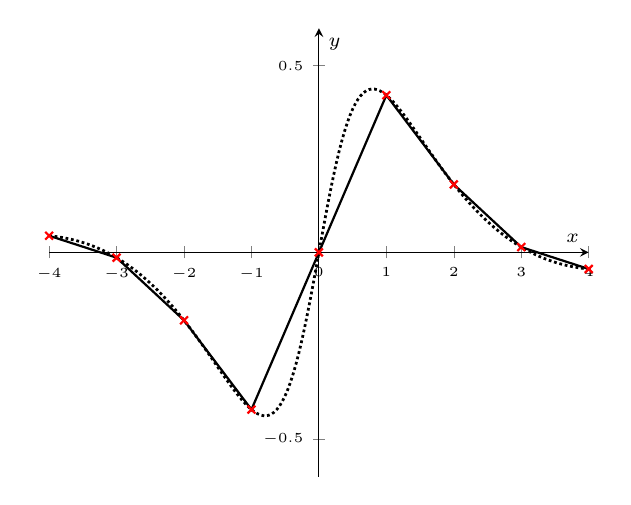
\begin{tikzpicture}[scale=1.0]
              \begin{axis}[axis lines=middle,xmin=-4.0,xmax=4.0,ymin=-0.6,ymax=0.6,
                xlabel=$\scriptstyle x$,
                ylabel=$\scriptstyle y$,
                xtick={-4, -3, -2, -1, 0, 1, 2, 3, 4},
                ytick={-0.5,0,0.5},
                extra x ticks={0},
                tick label style={font=\tiny},
                legend style={font=\small,legend pos=outer north east,}]
                \addplot[no marks,line width=1pt,black,domain=-4.0:4.0,samples=200,densely dotted] {(sin(deg(x)))/(1 + x^2)};
                \addplot[only marks,line width=2pt,red,domain=-4.0:4.0,samples=9, thick, mark=x] {(sin(deg(x)))/(1 + x^2)};
                \addplot[no marks,line width=2pt,black,domain=-4.0:4.0,samples=9, thick] {(sin(deg(x)))/(1 + x^2)};
              \end{axis}
            \end{tikzpicture}
        \end{center}

    \noindent Látható, hogy a lineáris spline jól közelíti a függvényt az egyes intervallumokon, kivéve a [-1, 1]-es intervallumot. Itt a függvény nem képes az eredeti görbületre illeszkedni.\\

    \noindent $p_{1}$ polinom az $[x_{0}, x_{1}]$ intervallumon.\\

    \begin{center}
        $p_{1}(x) = a_1^{(1)}(x - x_{0}) + a_{0}^{(1)}$\\
        $\boldsymbol{a_{0}} = f(-4) = -\ddfrac{sin(4)}{17}$\\
        $\boldsymbol{a_{1}} = \ddfrac{f(x_k) - f(x_{k-1})}{x_k - x_{k-1}} = \ddfrac{10 \sin(4) - 17 \sin(3)}{170}$
        $\boldsymbol{p_{1}(x)} = \ddfrac{10 \sin(4) - 17 \sin(3)}{170}x + \ddfrac{4(10 \sin(4) - 17 \sin(3))}{170} -\ddfrac{sin(4)}{17} = \ldots = \ddfrac{1}{170}\big( (10 sin(4) - 17 sin(3))x + 30 sin(4) - 68 sin(3) \big)$\\
    \end{center}

        \begin{center}
            \begin{tikzpicture}[scale=1.0]
              \begin{axis}[axis lines=middle,xmin=-4.0,xmax=-2.0,ymin=-0.1,ymax=0.1,
                xlabel=$\scriptstyle x$,
                ylabel=$\scriptstyle y$,
                xtick={-4,-3,-2},
                ytick={-0.1,0,0.1},
                extra x ticks={-3, -2},
                tick label style={font=\tiny},
                legend style={font=\small,legend pos=outer north east,}]
                \addplot[no marks,line width=1pt,black,domain=-4.0:-2.0,samples=50,densely dotted] {(1/(1 + x^2))*sin(deg(x))};
                \addlegendentry{$f(x)$}
                \addplot[only marks,line width=2pt,red,domain=-4.0:-3.0,samples=2, thick, mark=x] {(1/170)*(10*x*sin(deg(4))-17*x*sin(deg(3))+30*sin(deg(4))-68*sin(deg(3)))};
                \addplot[no marks,line width=2pt,black,domain=-4.0:-3.0,samples=2, thick] {(1/170)*((10*sin(deg(4))-17*sin(deg(3)))*x+30*sin(deg(4))-68*sin(deg(3)))};
                \addlegendentry{$x_{0},x_{1}$}
                \addlegendentry{$p_{1}(x)$}
              \end{axis}
            \end{tikzpicture}
        \end{center}
\centerline{\rule{17cm}{0.4pt}}
    \noindent Példa: Számoljuk ki, majd rajzoljuk fel az alábbi pontokra négyzetesen legjobban illeszkedő egyenest: $(x_1 = -1; y_1 =0) \quad (x_2 = 0; y_2 = 1) \quad (x_3 = 1; y_3 = 0) \quad (x_4 = 2; y_4 = 2)$ (legkisebb négyzetek módszere)

\begin{tabular}{p{0.48\textwidth} p{0.48\textwidth}}
    $A^{T}A = \begin{bmatrix}
        n & \sum\limits_{i=1}^{n}x_{i} \\[0.3em]
        \sum\limits_{i=1}^{n}x_{i} & \sum\limits_{i=1}^{n}x_{i}^{2} \\[0.3em]
    \end{bmatrix} =
    \begin{bmatrix}
        4 & 2 \\[0.3em]
        2 & 6 \\[0.3em]
    \end{bmatrix}$
&
    $A^{T}b = \begin{bmatrix}
        \sum\limits_{i=1}^{n}y_{i} \\[0.3em]
        \sum\limits_{i=1}^{n}x_{i}y_{i} \\[0.3em]
    \end{bmatrix} =
    \begin{bmatrix}
        3 \\[0.3em]
        4 \\[0.3em]
    \end{bmatrix}$
\end{tabular}

\begin{tabular}{p{0.48\textwidth} p{0.48\textwidth}}
    $A^{T}A\underline{a} = A^{T}\underline{b}$
&
    $\begin{bmatrix}
        4 & 2 \\[0.3em]
        2 & 6 \\[0.3em]
    \end{bmatrix} \cdot
    \begin{bmatrix}
        a_0 \\[0.3em]
        a_1 \\[0.3em]
    \end{bmatrix} =
    \begin{bmatrix}
        3 \\[0.3em]
        4 \\[0.3em]
    \end{bmatrix}$
\end{tabular}

    \begin{center}
        $4a_0 + 2a_1 = 3 \Rightarrow 4a_0 = 3 - 2a_1 \Rightarrow a_0 = \ddfrac{3-2a_1}{4}$ \\
        $2a_0 + 6a_1 = 4 \Rightarrow 2 \cdot \ddfrac{3-2a_1}{4} + 6a_1 = 4 \Rightarrow 3 - 2a_1 + 12a_1 = 8 \Rightarrow 10a_1 = 5 \Rightarrow a_1 = \ddfrac{1}{2}$ \\
        $a_0 = \ddfrac{3 - 2 \cdot \ddfrac{1}{2}}{4} = \ddfrac{1}{2}$
    \end{center}

    \noindent A megoldás: $l(x) = \ddfrac{1}{2}x + \ddfrac{1}{2}$

    \begin{center}
        \begin{tikzpicture}[scale=1.0]
          \begin{axis}[axis lines=middle,xmin=-2.0,xmax=3.0,ymin=-2.0,ymax=5.0,
            xlabel=$\scriptstyle x$,
            ylabel=$\scriptstyle y$,
            tick label style={font=\tiny},
            legend style={font=\small,legend pos=outer north east,}]
            \addplot[no marks,line width=2pt,blue,domain=-2.0:3.0,samples=100, thick] {(1/2)*x + 1/2};
            \addplot[only marks,color=black,thick,mark=*, mark options={fill=red}]
    coordinates {
         (-1, 0)
         (0, 1)
         (1, 0)
         (2, 2)
        };
          \end{axis}
        \end{tikzpicture}
    \end{center}
\end{document} 